% !TEX encoding = UTF-8 Unicode
% !TEX TS-program = pdflatex
\PassOptionsToPackage{corpo=12pt,tipotesi=magistrale,numerazioneromana}{toptesi}
\documentclass[a4paper,12pt,oneside]{toptesi}
\input{common/packages}
\usepackage{longtable}
\usepackage{xurl}
\input{common/package_config}
\input{common/new_commands}
% Title-page information supplied by the author.
\newcommand{\thesistitle}{Adaptive Granularity Retrieval for Retrieval-Augmented Generation}
\newcommand{\thesissubtitle}{}
\newcommand{\thesiscandidatename}{Niusha}
\newcommand{\thesiscandidatesurname}{Parsa}
\newcommand{\thesissupervisoronename}{Professor Giuseppe}
\newcommand{\thesissupervisoronesurname}{Rizzo}
\newcommand{\thesissupervisortwoname}{Dr. Lorenzo}
\newcommand{\thesissupervisortwosurname}{Bongiovanni}
\newcommand{\thesisdate}{September 2026}
\newcommand{\thesiscourse}{Master's Degree in Data Science and Engineering}
\newcommand{\academicYear}{Academic Year 2025--2026}
\newcommand{\thesisuniversity}{Politecnico di Torino}
\newcommand{\thesiscandidatetext}{Candidate}
\newcommand{\thesissupervisortext}{Supervisors}

\input{common/font_config}
\addbibresource{references.bib}
\hypersetup{pdftitle={Adaptive Granularity Retrieval for Retrieval-Augmented Generation},
  pdfauthor={Niusha Parsa},pdfsubject={Master's thesis, Data Science and Engineering}}
\newcommand{\granularities}{\mathcal{G}}
\newcommand{\retrievalf}{F_{\mathrm{ret}}}
\begin{document}
\overfullrule=0pt
\emergencystretch=2em
\raggedbottom
\setlist[description]{labelwidth=0pt,labelsep=0pt}
\setcounter{tocdepth}{2}
\setcounter{secnumdepth}{2}
\renewcommand{\topfraction}{0.85}
\renewcommand{\bottomfraction}{0.65}
\renewcommand{\textfraction}{0.10}
\renewcommand{\floatpagefraction}{0.75}
\setcounter{totalnumber}{3}

\english
\hypersetup{pageanchor=false}
% Personal details belong in thesis_info.tex.
\newgeometry{top=2.8cm,left=2.8cm,right=2.8cm,bottom=2.8cm,heightrounded}
\begin{titlepage}
\centering
\includegraphics[width=105mm]{\thesisuniversitylogo}\par
\vspace{1.2cm}
{\institutionfont\textbf{\thesisuniversity}\par}
\vspace{0.8cm}
{\large\thesiscourse\par}
\vspace{0.3cm}
{\large\academicYear\par}
{\large Graduation Session: \thesisdate\par}
\vfill
{\customtitlefont\textbf{\thesistitle}\par}
\vfill
\begin{minipage}[t]{0.61\textwidth}
\raggedright
{\large\textbf{\thesissupervisortext}\par}
\medskip
{\large\thesissupervisoronename\ \thesissupervisoronesurname\par}
{\large\thesissupervisortwoname\ \thesissupervisortwosurname\par}
\end{minipage}\hfill
\begin{minipage}[t]{0.32\textwidth}
\raggedright
{\large\textbf{\thesiscandidatetext}\par}
\medskip
{\large\thesiscandidatename\ \thesiscandidatesurname\par}
\end{minipage}
\vspace{1cm}
\end{titlepage}
\restoregeometry

\frontmatter
\pagenumbering{roman}
\hypersetup{pageanchor=true}
\chapter*{Abstract}
\addcontentsline{toc}{chapter}{Abstract}
Retrieval-augmented generation depends on finding useful evidence. The
size of the passages available for retrieval is often fixed before a
question is seen, even though different questions may need different
amounts of context. Short passages can isolate a detail but lose its
surroundings; longer passages can preserve context while introducing
irrelevant material. This thesis investigates whether adapting retrieval
granularity, the size of the retrieved chunks, improves evidence recovery
within a known source document.

The study uses QASPER scientific papers, five chunk sizes from 10 to 160
GPT-2 tokens, and fixed dense embeddings. The question-level experiments
use 2,245 training questions and 924 validation questions, with five
chunks retrieved from the associated paper. Methods progress from fixed
and mixed sizes through question-embedding and Qwen routers to similarity
trees, out-of-fold feature fusion, expected-regret learning, and local
routing. Evaluation measures lexical overlap with annotated evidence
using joined evidence-token F1.

Fixed 40-token retrieval achieves mean F1 of 0.3159. An offline oracle
that uses the reference evidence to choose the best of the five saved
results per question reaches 0.3821. The strongest learned question-level
method, expected-regret routing, reaches 0.3075, remaining below the fixed
baseline. Local routing reaches 0.3053, compared with 0.3075 for a
fixed-40 baseline using the same selected trees. Adding a frozen Qwen
context-need feature gives 0.3045, with no demonstrated improvement.

The results show that better prediction of evidence length does not
reliably translate into better retrieval. Learning from retrieval regret
produces the strongest tested global router, but the study finds no
demonstrated advantage over the corresponding fixed-size baselines.
The findings concern evidence retrieval; generated-answer quality remains
unevaluated. Repeated use of validation data during development also
limits claims about performance on unseen data.

\chapter*{Summary}
\addcontentsline{toc}{chapter}{Summary}
A retrieval system must decide how much text to return as one passage.
A question asking for a dataset name may need only a short phrase,
while an explanation may require several connected statements. A longer
passage can preserve useful context, but it can also bury the relevant
detail in unnecessary material.

This thesis asks whether adapting chunk size to a question or a region
of a paper recovers evidence more effectively than using one size
throughout. The study focuses on the retrieval stage of
retrieval-augmented generation (RAG). It evaluates evidence selection;
generated answers are outside its scope.

The experimental environment was built around QASPER, a dataset of
questions about scientific papers. Each paper was represented at five
granularities: 10, 20, 40, 80, and 160 GPT-2 tokens, using fixed
\texttt{text-embedding-3-small} embeddings stored in Qdrant. Retrieval
was restricted to the associated paper, isolating evidence selection
from document discovery.
The frozen question-level population contains 2,245 training questions
and 924 validation questions. The main retrieval protocol returns five
chunks per question. Its primary metric, joined evidence-token F1,
measures lexical overlap between the combined retrieved text and the
annotated evidence.

The work began with a Weaviate prototype before moving to Qdrant.
Resumable ingestion and checks of identifiers, offsets, and collection
completeness established a consistent experimental pipeline.

Fixed-size retrieval provided the main reference. Among the five sizes,
40 tokens achieved the highest mean joined retrieval F1, 0.3159. The
offline best-size oracle achieved 0.3821 by using the reference evidence
to select among all five retrieval outcomes. This gap shows that different
questions can benefit from different sizes. It does not establish that
a router can predict those choices for a new question.

The early adaptive methods used the question embedding to predict a size,
or pooled chunks from all sizes into a single ranking. The selected
logistic-regression router reached 0.2853 retrieval F1. Raw mixed-size
retrieval reached 0.2562, and overlap-aware deduplication raised this to
0.2618. Both mixtures remained below fixed 40 and favoured short chunks,
even after deduplication.

\newpage
The next experiments asked whether a small Qwen model could make a better
decision from the question wording. They covered zero-shot prompting,
numeric-output fine-tuning, restricted alias classification, class-balanced
loss, a dedicated classification head, explicit token-count instructions,
and a learning-rate and training-duration search. The strongest
Qwen-only retrieval result was 0.2865 when fine-tuning the model to choose
among five single-token labels with uniform loss weights. Numeric
fine-tuning increased label accuracy while favouring
large chunks and reducing retrieval F1. The contrast exposed a weakness
of the target: total evidence length does not necessarily identify the
best size for each of five retrieved chunks.

The study then added information from the document. Similarity trees
describe how question-to-chunk scores change between aligned coarse and
fine spans. Linear classifiers and boosted trees were evaluated on
level-wise and hierarchical features, followed by fusion with Qwen
features. The initial fusion used Qwen predictions on examples that had
trained the base model. A corrected run used paper-grouped out-of-fold
predictions: each training paper was predicted by a model fitted on other
papers. This removed the known contamination in the training features.
Corrected fusion reached 0.2783 retrieval F1, below the original result.

The strongest learned question-level method used expected-regret
regression. It learned the loss in retrieval F1 associated with each
size, making supervision reflect the consequences of a routing decision.
It reached 0.3075 mean retrieval F1, ahead of the preceding learned
routers. Its difference from fixed
40-token retrieval was $-0.00835$, with a paired paper-cluster bootstrap
95\% interval of $[-0.01266,-0.00416]$. Within the evaluated development
sample, the fixed baseline remained stronger.

Finally, local routing allowed different regions of the same paper to use
different sizes. The router learned from 4,081 question--tree examples
drawn from 2,101 questions with mappable evidence. At inference, it chose one
size within each of the five highest-ranked 160-token trees and returned
one chunk per tree.
This reached 0.3053 F1, against 0.3075 for a fixed-40 method using the same
trees. A frozen Qwen feature describing the anticipated context need as
short, medium, or long was also tested. Free generation sometimes
produced answers instead of a category. Restricting the decision to
the three labels resolved that problem, but almost every question
received \enquote{medium}. Retrieval
F1 was 0.3045, with no demonstrated gain over the local router alone.

The experiments identify retrieval-utility supervision as a promising
direction, without demonstrating an advantage over the corresponding
fixed baselines. Comparisons also depend on the returned text budget:
five chunks can contain very different amounts of text. Since validation
informed repeated development decisions, the next step is evaluation on
untouched data, followed by additional datasets and measurements of
generated-answer quality.

% Personal acknowledgements are intentionally omitted until supplied by the author.
\tableofcontents
\listoftables
\listoffigures
\chapter*{Abbreviations and notation}
\addcontentsline{toc}{chapter}{Abbreviations and notation}
\begin{tabularx}{\textwidth}{@{}lX@{}}
\toprule
Term & Meaning in this thesis\\
\midrule
RAG & Retrieval-augmented generation\\
NLP & Natural language processing\\
LLM & Large language model\\
GPT-2 & Tokenizer used for chunk boundaries and lexical evaluation\\
QASPER & Question-answering dataset over scientific research papers\\
OOF & Out-of-fold: a prediction made by a model not fitted on that fold\\
SFT & Supervised fine-tuning\\
MLP & Multilayer perceptron\\
HNSW & Hierarchical navigable small world vector index\\
$q,d$ & Question and its associated source paper\\
$\granularities$ & Candidate chunk sizes $\{10,20,40,80,160\}$ tokens\\
$K$ & Number of retrieved chunks; $K=5$ in the primary protocols\\
$s(q,c)$ & Cosine similarity between a question and a chunk\\
$E(q)$ & Joined reference evidence for a question\\
$R_g(q)$ & Ranked top-$K$ chunks retrieved at size $g$\\
$U(q,g)$ & Joined retrieval token F1 for $R_g(q)$\\
$C(q,g)$ & Regret relative to the best of the five fixed-size actions\\
\bottomrule
\end{tabularx}

\medskip
\enquote{Validation} names the repository split. Because that split was consulted
throughout development, its results are interpreted as development-set
findings, not as a final, untouched test evaluation. \enquote{Classification F1}
and \enquote{retrieval F1} refer to different tasks and are kept separate.

\mainmatter
\chapter{Introduction}
\label{ch:introduction}

\section{Motivation}
A useful answer often depends on a small part of a much larger document.
Finding that part is not just a matter of choosing the right document.
Even after the source is known, a retrieval system must decide what to
return from it. A phrase may identify a method, a paragraph may explain
its assumptions, and several passages may be needed to compare the
results of two experiments. The unit of retrieval therefore shapes what
an answering system can see.

Retrieval-augmented generation (RAG) brings retrieved material into the
generation process instead of relying only on information stored in a
model's parameters \cite{lewis2020rag}. This creates a useful separation
between acquiring evidence and producing an answer, but it also gives
the retrieval stage considerable responsibility. If relevant text is
missing, the generator has to work without it. If the supplied text is
mostly irrelevant, the generator must distinguish the useful evidence
from the surrounding material. Good retrieval is not sufficient for
good generation, but it is a necessary part of a dependable pipeline.

Chunking is one of the decisions that connects those two stages. In
fixed-size chunking, a document is divided into pieces according to a
token budget selected in advance. The same rule applies to all questions,
including those that need very different amounts of evidence. This is
convenient: indexing is straightforward, every chunk has a predictable
nominal size, and the retrieval procedure has few moving parts. It is
less clear whether that convenience comes at the expense of evidence
quality.

The intuition behind adaptive granularity is simple. Rather than ask
every question to work with the same chunk size, allow the system to
select a size that suits the current information need. The difficulty is
knowing what \enquote{suits} means before the answer is available. A
question may sound broad while its evidence is concentrated in one
sentence. A short factual question may depend on a table or on several
parts of a paper. Even a correct estimate of the total evidence length
does not specify how that evidence is distributed across retrievable
pieces.

Scientific papers make this problem particularly interesting. They
contain definitions, methodological explanations, experimental settings,
and results, often spread across separate sections. QASPER provides
questions anchored in such papers together with annotated supporting
evidence \cite{dasigi2021qasper}. This allows the granularity decision to
be studied against an explicit evidence target rather than against an
informal impression of what a passage should contain.

\section{Problem statement and scope}
This thesis asks whether an adaptive choice of chunk size can improve
evidence retrieval within a known source paper. The candidate sizes are
$\granularities=\{10,20,40,80,160\}$ GPT-2 tokens. The primary
question-level protocol selects one size and retrieves the five most
similar chunks at that size. Later experiments make the decision locally,
allowing different regions of the same paper to contribute chunks at
different sizes.

This is a deliberately controlled problem. The source paper is supplied
by the dataset, embeddings remain fixed, and retrieval uses cosine
similarity. The experiments do not train an embedding model, search an
unknown corpus for the correct paper, rerank passages with a cross-encoder,
or generate final answers. These choices isolate the granularity decision
and make its successes and failures easier to interpret.

The main outcome is joined evidence-token F1: the lexical overlap between
the combined retrieved text and the combined annotated evidence.
Chapter~\ref{ch:data} defines the metric precisely. Throughout the thesis,
\emph{retrieval F1} refers to this measure. It is distinct from the
classification F1 used to assess predicted size labels, and from the
answer-level scores used in a complete question-answering system.

The word \emph{adaptive} also needs a boundary. A method is adaptive here
when its size choice depends on the question or its similarity pattern
within the paper. An offline oracle that inspects gold evidence is not
a deployable adaptive method. It provides a reference for what could be
gained if the best of the available actions were known. Likewise, a
method that retrieves many more chunks is not automatically better
adaptation; it may simply spend a larger context budget.

\section{Research questions}
The investigation is organised around five research questions.

\begin{description}[style=nextline,leftmargin=0pt]
\item[RQ1: Is there useful headroom beyond a fixed granularity?]
How do the five fixed sizes compare, and how much can an offline
per-question choice improve over the strongest fixed setting?
\item[RQ2: Can the question alone support a useful size decision?]
Do question embeddings or a small language model predict a granularity
that improves evidence retrieval? How closely does label prediction
track the retrieval outcome?
\item[RQ3: Does the document's similarity structure add information?]
Can score distributions across coarse and fine spans help a router?
Does combining those signals with language-model features improve the
decision when stacking is trained without in-sample base predictions?
\item[RQ4: Is direct retrieval-utility supervision more effective?]
What changes when the target becomes the cost of a retrieval decision
rather than an evidence-length class?
\item[RQ5: Does local adaptation improve a matched retrieval pipeline?]
Can a system benefit from selecting different sizes in different regions,
and does a frozen language-model estimate of context need add useful
information to that local decision?
\end{description}

These questions reflect the actual development of the project. They are
not five independent confirmations of a single preselected method. The
answer to one question often motivated a change in the next experiment.
That history is important because it explains both the design choices
and the limits of the final evaluation.

\section{Experimental approach}
The work began with data ingestion and a fixed retrieval benchmark.
Documents were represented at all five sizes, embedded, and stored with
stable identifiers and source offsets. Questions and evidence were
normalised and audited. Fixed-size retrieval established the reference
outcomes from which oracle labels and later utility targets could be
constructed.

The first learned router used the question embedding. Logistic regression
and a small multilayer perceptron tested whether a comparatively cheap
representation was already sufficient. Mixed-size retrieval tested a
different possibility: perhaps it was unnecessary to predict a size at
all if candidates from all levels could share one ranking. These methods
provided practical baselines before introducing a language model.

The Qwen sequence then investigated the question-only decision in more
detail. It moved from frozen prompting to supervised numeric generation,
restricted alias outputs, class weighting, and a dedicated classification
head. A prompt change and a small learning-rate grid examined whether
the remaining limitation was primarily the output interface or the
training configuration.

The next sequence used the evidence landscape without using gold
evidence at inference. Similarity-tree features describe where high
question-to-chunk scores occur and whether they persist across scales.
Linear models, boosted trees, and Qwen-feature fusion were evaluated.
The fusion procedure was then corrected to use paper-grouped out-of-fold
base predictions, making the training interface closer to the way the
fusion model would encounter a new question.

Finally, expected-regret learning changed the objective, while local
routing changed the decision unit. A frozen short/medium/long Qwen feature
was added to the local router in the last experiment. Its unsuccessful
free-generation version and its constrained-output replacement are both
part of the record.

\section{Contributions}
The contribution is an evidence-based study of the granularity decision,
rather than a claim that one adaptive architecture universally solves it.
Four aspects of the work are particularly useful.

First, the repository provides a reproducible multi-granularity evaluation
setting with frozen questions, fixed embeddings, paper-restricted retrieval,
versioned metrics, and recoverable intermediate outputs. This makes it
possible to compare substantially different routers against the same
underlying retrieval actions.

Second, the study separates several meanings of an oracle. The
retrieval-optimal action, the total evidence-length category, and the
local evidence-overlap category supervise different decisions. Making
those differences explicit explains why classification improvements
sometimes move retrieval in the wrong direction.

Third, the experiments include methodological corrections and negative
results. In particular, the out-of-fold fusion rerun and the invalid-output
gate in the final Qwen feature experiment expose failure modes that would
be easy to hide in a report containing only the best scores.

Fourth, the expected-regret and matched local-routing comparisons identify
where adaptation became more competitive and where it still fell short.
The strongest learned question-level router reached 0.3075 mean retrieval
F1, but fixed 40-token retrieval reached 0.3159. Local routing similarly
did not demonstrate an advantage over its matched fixed-40 comparator.
These results support a more precise conclusion than either
\enquote{adaptation works} or \enquote{adaptation is unnecessary}.

\section{How to read the findings}
The repository's validation split was consulted across successive modelling
decisions. Although several later protocols use training-only selection,
prediction locks, and grouped folds, these safeguards cannot turn a
repeatedly observed validation split into an untouched test set. The
reported comparisons are therefore development findings. Their confidence
intervals quantify resampling uncertainty within the observed papers,
not all uncertainty due to model selection, random seeds, or transfer to
another domain.

This distinction does not make the experiments uninformative. It changes
what can be concluded from them. A carefully controlled improvement over
an earlier router can motivate the next study, while a final superiority
claim requires independent confirmation. The thesis keeps both ideas in
view: the results are useful, and their evidential scope is limited.

\section{Thesis organisation}
Chapter~\ref{ch:background} introduces the retrieval concepts and places
the work alongside research on granularity, hierarchy, and adaptive RAG.
Chapter~\ref{ch:data} describes QASPER, preprocessing, data integrity, and
evaluation targets. Chapter~\ref{ch:method} develops the baseline and
adaptive methods in experimental order. Chapter~\ref{ch:results} presents
the results, controlled comparisons, unsuccessful runs, and threats to
validity. Chapter~\ref{ch:conclusion} answers the research questions and
sets out the next experiments needed for a stronger conclusion. The
appendices document the chronology, configurations, output contracts,
and links between reported results and repository artifacts.

\chapter{Background and Literature Review}
\label{ch:background}

\section{Retrieval as part of an answering system}
A language model can produce a fluent answer without exposing where its
information came from. Retrieval offers a different interface: relevant
external text is selected and made available to the answering model.
Lewis et al.\ formalised a RAG architecture combining a retriever with a
sequence-to-sequence generator, bringing non-parametric information into
the prediction process \cite{lewis2020rag}. In this thesis, that broader
architecture motivates the task, but only the evidence-selection stage
is evaluated.

Retrieval itself has several decisions. The system needs a searchable
representation, a relevance function, a candidate set, and a rule for
constructing the final context. Granularity affects all four. Changing
the boundaries of a passage changes its embedding, the number of indexed
items, the competition between candidates, and the amount of text returned
for a fixed number of results. It is therefore more than a formatting
choice made after retrieval.

It is helpful to distinguish document retrieval from passage retrieval.
In an open-domain setting, finding the relevant document is part of the
task. In this study, the associated QASPER paper is known and retrieval
is filtered to that paper. The remaining difficulty is selecting evidence
inside it. A method that succeeds under this restriction may still fail
when unrelated documents are introduced, because the score distributions
and the nature of hard negatives change.

\section{Dense representations and similarity search}
Dense retrieval maps questions and passages into a vector space. A
similarity function then ranks passages by their relation to the question.
Dense Passage Retrieval demonstrated the effectiveness of learned
question and passage encoders for open-domain question answering
\cite{karpukhin2020dpr}. The present project uses a fixed embedding
service rather than retraining such a retriever. Consequently, any
improvement must come from selecting or organising the existing
representations, not from learning a better embedding space.

For nonzero vectors $\mathbf{e}_q$ and $\mathbf{e}_c$, cosine similarity is
\begin{equation}
s(q,c)=\frac{\mathbf{e}_q^\top\mathbf{e}_c}
{\|\mathbf{e}_q\|_2\|\mathbf{e}_c\|_2}.
\label{eq:cosine}
\end{equation}
The repository uses \texttt{text-embedding-3-small} with 1,536-dimensional
vectors \cite{openai2024embeddings}. It keeps the model and dimension
fixed across the reported retrieval comparisons. This controls an
important source of variation, although it also limits the conclusions
to one embedding representation.

Qdrant stores vectors together with payload fields used for filtering,
including paper identity and granularity \cite{qdrantcollections}.
Its vector index is an infrastructure component, not the document
hierarchy proposed later in the thesis. HNSW organises vectors for
approximate nearest-neighbour search \cite{malkov2016hnsw}; the
similarity tree in this work organises aligned text spans within a
paper. The two structures solve different problems despite both using
hierarchical organisation.

A high cosine score should not be read as a calibrated probability that
a passage contains sufficient evidence. In particular, scores produced
for different passage lengths may have different distributions. The
mixed-size experiments directly test what happens when those scores
are pooled without learning a cross-granularity calibration. Their
outcome is therefore informative about this pipeline, but it is not a
general theorem about dense retrieval.

\section{What retrieval granularity changes}
\subsection{Precision, coverage, and context}
A small chunk can concentrate on words closely related to a question.
It can also cut away a definition, a qualifier, or the subject of a
pronoun. A large chunk can retain those connections while bringing in
text that does not belong to the evidence. Neither choice is uniformly
better. The right balance depends on the scoring objective as well as
the document.

In a top-$K$ evaluation, length and count interact. With five full chunks,
10-token retrieval returns approximately 50 source tokens, whereas
160-token retrieval returns approximately 800. The two methods have
the same number of results but not the same text budget. A rise in recall
at the larger size may simply reflect this increase in coverage.
Likewise, a decline in precision may reflect the additional denominator
in the lexical metric. A fair interpretation must retain both facts.

Evidence annotations introduce a further distinction. The number of
tokens highlighted by an annotator describes the reference material,
not necessarily the best size of an independently ranked chunk. If
evidence consists of several short statements, retrieving several
compact chunks may be preferable to retrieving several long chunks
whose length resembles the total annotation. This observation motivates
the later move from evidence-length classification to retrieval regret.

\subsection{Fixed windows and semantic units}
Fixed token windows are simple and reproducible, but their boundaries
need not match sentences or propositions. Dense X Retrieval studies
retrieval units at several levels and argues for propositions as atomic,
self-contained pieces of information \cite{chen2024densex}. Its units
are constructed semantically. A 10-token window in this project is not
equivalent to a proposition, and the thesis does not claim to reproduce
that method.

The advantage of the fixed windows here is experimental alignment. The
chosen sizes double at each level, so a coarse window contains smaller
windows from the same token sequence. This makes parent--child score
comparisons possible without an additional sentence segmentation or
semantic clustering procedure. The disadvantage is equally concrete:
the resulting hierarchy preserves positional containment, not
necessarily a meaningful discourse structure.

An alternative way to retain context is to change when embeddings are
constructed. Late Chunking encodes a longer text before pooling token
representations into chunk embeddings, allowing the chunk representation
to retain surrounding context \cite{gunther2024late}. The repository
instead embeds each stored chunk as its own text. The current results
therefore do not answer whether adaptive routing remains useful when
small chunks already have contextualised representations.

\section{Hierarchical retrieval}
Hierarchical approaches offer access to information at more than one
scale. RAPTOR recursively groups and summarises text to build a
tree-organised retrieval structure \cite{sarthi2024raptor}. Its upper
levels contain generated summaries. The hierarchy in this thesis is
different: a 160-token node is a literal span of the paper, not an
abstraction generated from its descendants. This avoids an extra
summarisation model and preserves direct source offsets.

The distinction matters for both capability and evaluation. A generated
summary can express information not present in any single child and can
combine evidence across separated parts of a document. A contiguous
token tree cannot do that. On the other hand, its parent and child
spans have a transparent containment relation, making it possible to
measure local overlap with annotated evidence and to inspect score
differences without assessing summary faithfulness.

The similarity-tree hypothesis is that these score differences reveal
something about evidence concentration. A strong parent and consistently
strong children may suggest a broadly relevant region. A single strong
child among weak siblings may suggest a narrow match. This is an
interpretation of possible signals, not an assumption that either
pattern always identifies gold evidence. The experiments test whether
a classifier can use these patterns more effectively than it uses
level-wise score summaries alone.

\section{Adaptive retrieval in RAG}
Adaptation can occur at several points in a retrieval pipeline.
Adaptive-RAG uses question complexity to select among answering
strategies with different retrieval demands, including different
amounts of retrieval activity \cite{jeong2024adaptive}. Its decision is
about the retrieval strategy, rather than choosing among the five
fixed token lengths used here. The shared idea is that a question can
inform how resources are allocated; the action spaces and supervision
are different.

Self-RAG integrates decisions to retrieve with generation and
self-reflection through special reflection tokens
\cite{asai2023selfrag}. It addresses the interaction between retrieval,
generation, and critique. This thesis keeps generation outside the
evaluation and makes a narrower decision before evidence is returned.
A successful router here would therefore be a possible retrieval
component, not a replacement for a system that verifies its generated
claims.

Mix-of-Granularity (MoG) is a particularly close reference point for
the present study. It uses a learned router to select retrieval
granularity from the input query instead of applying one fixed
granularity to every query, and trains that router with soft-label
supervision \cite{zhong-etal-2025-mix}. Its graph extension,
MoG-Graph (MoGG), reorganises documents as graphs so that relevant
pieces that are non-adjacent in the original text can be retrieved
through graph neighbourhoods. The present thesis does not reproduce
MoG or MoGG. It instead studies evidence retrieval within a known
QASPER source paper, using aligned fixed GPT-2 token spans at sizes
$\{10,20,40,80,160\}$. Its primary outcome is joined evidence-token
retrieval F1 rather than generated-answer accuracy, and it compares
evidence-length classification, question-only Qwen routing,
similarity-tree features, and direct retrieval-regret supervision.

The amount of supplied context also cannot be separated entirely from
how a generator uses it. Lost in the Middle reports sensitivity to the
position of relevant information in long contexts
\cite{liu2023lost}. This motivates care in assembling evidence, but
does not establish that a higher lexical retrieval F1 will produce
better answers in the present setting. That connection requires a
downstream experiment with a specified generator and context ordering.

\begin{table}[tbp]
\centering\small
\caption{Position of the thesis relative to neighbouring retrieval ideas.
The rows describe different decisions, not a ranking of methods.}
\label{tab:literature}
\begin{tabularx}{\textwidth}{@{}p{3.1cm}XX@{}}
\toprule
Approach & Main decision or representation & Difference from this thesis\\
\midrule
Dense X Retrieval & Semantic retrieval units, including propositions & Fixed token spans are not semantic propositions\\
RAPTOR & Hierarchy with recursively generated summaries & Trees here contain literal, aligned source spans\\
Late Chunking & Contextualise before forming chunk embeddings & Stored chunks here are embedded independently\\
Adaptive-RAG & Adapt the answering/retrieval strategy & The primary action here is chunk size\\
Self-RAG & Retrieve, generate, and critique jointly & Only evidence retrieval is evaluated here\\
Mix-of-Granularity (MoG) & Query-dependent routing across retrieval granularities & Medical QA; here, compare routing targets, including retrieval utility, over aligned token spans within a known QASPER paper\\
This work & Select global or local token granularity & Compare decisions under fixed embeddings and explicit evidence scoring\\
\bottomrule
\end{tabularx}
\end{table}

\section{Learning a router}
\subsection{Classification and its target}
A router can be expressed as a classifier over five sizes. Given features
$\mathbf{x}$, it predicts probabilities $p_\theta(g\mid\mathbf{x})$ and
chooses the largest. Standard cross-entropy rewards the labelled size
and penalises every other size through the same categorical objective.
Its suitability depends on how that label was obtained.

If the target is evidence length, a correct classification means that
the model has recovered a length category. It does not mean that the
associated top-five retrieval set is optimal. If two sizes have almost
identical retrieval utility, a hard label also hides that similarity.
Conversely, two equally wrong classifications can have very different
retrieval costs. These are objective-design issues, not simply limits
of classifier capacity.

Class imbalance creates an additional difficulty. Class-balanced loss
uses the effective number of samples to reduce the dominance of common
classes \cite{cui2019classbalanced}. This provides the weighting
principle tested in Phase 2B. It cannot, by itself, make a proxy target
more faithful to the downstream retrieval objective.

\subsection{Nonlinear models and combined features}
Boosted decision trees provide a way to learn nonlinear interactions
between score statistics without fine-tuning the embedding model.
XGBoost supplies a regularised gradient-boosting implementation
\cite{chen2016xgboost}. Here its role is modest: learn whether particular
combinations of level-wise and hierarchical features support a size
decision. Feature importance can suggest which measurements the fitted
model used, but it does not establish a causal explanation of relevance.

Combining a language model and a tree model raises a separate training
question. If a second-stage learner sees base-model predictions on
examples that trained the base model, its inputs can be unrealistically
confident. Out-of-fold predictions are a practical way to reduce this
mismatch. Grouping by paper is important because questions about the
same paper share content and should not be treated as independent
documents when constructing the folds.

\section{Evaluation as part of the method}
Evaluation is not a final reporting step detached from model design.
The target, decision unit, candidate set, and retrieval budget determine
what a score means. A question-level classifier, a local-tree classifier,
and a retrieval system can all report an F1 value while measuring
different events.

Uncertainty also depends on the unit of observation. Questions from the
same paper share a source, so resampling individual questions can ignore
an important dependence. The later repository comparisons resample
papers and preserve all of their questions. General guidance on
significance testing in NLP emphasises choosing procedures that match
the task and comparison \cite{dror2018testing}. The exact paired
paper-cluster bootstrap used here is specified in
Chapter~\ref{ch:results}.

The gap addressed by this thesis is consequently specific. It is not
that granularity or adaptive retrieval has never been studied. It is
the empirical question of which signals and learning targets support
a useful granularity choice in this fixed, evidence-annotated setting,
and whether their added complexity beats a strong fixed-size baseline.

\chapter{Dataset and Preprocessing}
\label{ch:data}

\section{QASPER and the experimental population}
QASPER contains 5,049 information-seeking questions associated with 1,585
NLP research papers, with answers and supporting evidence annotations
\cite{dasigi2021qasper}. This structure makes it possible to evaluate
retrieval against evidence from a known source. It also introduces
practical complications: papers have different lengths, questions can
have multiple annotations, and some evidence refers to tables or figures
that do not have a directly recoverable text span.

The published dataset size is not the denominator used in every
repository experiment. The frozen supervised population contains 2,245
training questions from 845 papers and 924 validation questions from
277 papers. Those are the counts used for the main question-level
comparisons. They describe the preserved, eligible experimental records,
not a claim that every original question has usable text evidence for
every later method.

\begin{table}[tbp]
\centering
\caption{Populations used in the main experiments. The local training
rows are derived from the frozen question-level training population.}
\label{tab:populations}
\begin{tabularx}{\textwidth}{@{}Xrr@{}}
\toprule
Population & Questions & Papers\\
\midrule
Frozen question-level training & 2,245 & 845\\
Frozen validation retrieval & 924 & 277\\
Eligible local-router training & 2,101 & ---\\
Excluded from local training: no mappable text evidence & 144 & ---\\
\bottomrule
\end{tabularx}
\end{table}

The same paper must not appear on both sides of a grouped training
fold. The later five-fold procedures therefore group questions by
paper identifier. Validation remains outside those training folds.
However, it was used repeatedly across the development sequence,
including checkpoint selection in the Qwen experiments. This thesis
does not report a final test-set evaluation.

\section{Document construction and token boundaries}
\subsection{Flattening the source}
The ingestion code constructs a single paper text from the title,
abstract, section names, and section paragraphs. Nonempty components
are joined with double newlines. Retaining section names gives the
retriever access to signals such as an experimental or methodological
heading, while the single source string provides a consistent coordinate
system for chunk and evidence offsets.

This representation is a text view of a scientific paper, not a
reconstruction of its PDF layout. A table may be represented differently
from its appearance on the page, and figure-based evidence may not be
locatable as ordinary prose. The method should therefore be understood
as text evidence retrieval over the dataset's representation.

\subsection{Five aligned granularities}
The GPT-2 fast tokenizer is applied without special tokens and with
offset mappings. For a token sequence of length $L$, a size $g$ defines
successive ranges
\begin{equation}
[jg,\min((j+1)g,L)),\qquad
j=0,\ldots,\left\lceil L/g\right\rceil-1.
\label{eq:chunks}
\end{equation}
The final chunk may be shorter than $g$. The source text for a chunk is
sliced using the corresponding character offsets. Thus the stored
content can be traced to the flattened paper rather than reconstructed
from a potentially different token decoder.

Chunks do not overlap within a level. Because all sizes are multiples
of ten and double successively, boundaries align in token space across
levels. A complete 160-token root contains two 80-token children, four
40-token descendants, eight 20-token descendants, and sixteen 10-token
leaves. At document edges the tree can be partial. This alignment
supports the later hierarchy without implying that every boundary
coincides with a sentence or that every inter-token whitespace character
belongs to a stored span.

Token counts used for boundaries must also be distinguished from counts
after joining or normalising retrieved text. Joining separately sliced
chunks can change tokenisation at boundaries. For this reason, reported
retrieved token counts need not equal exactly five times the nominal
chunk size, even before considering short final chunks.

\section{Embedding and storage}
The project embeds questions, chunks, and evidence using
\path{text-embedding-3-small}, with 1,536 dimensions. Qdrant contains
three relevant collections: \texttt{PaperChunk},
\texttt{PaperQuestion}, and \texttt{PaperEvidence}. Payloads retain
identities, split information, chunk size, and available source offsets.
Granularity is a filter within the chunk collection; the five levels
should not be mistaken for five unrelated embedding models.

A read-only collection audit recorded 1,701,822 chunks, 4,526 questions,
and 9,522 evidence records. These are storage counts across the ingested
material. They are not the frozen training and validation sample sizes
in Table~\ref{tab:populations}. In particular, the presence of other
split records in storage does not imply that a test benchmark was
evaluated in the thesis.

The embedding pipeline batches requests, retries failures, and preserves
the association between input texts and returned vectors. Stable UUID5
identifiers are derived from document, granularity, and chunk index for
chunks; evidence identity incorporates its text hash. This allows
repeated ingestion to upsert the intended objects rather than silently
creating additional copies.

The Qdrant setup uses cosine distance, on-disk vector storage, HNSW,
and payload indexes for common filters. A historical audit recorded a
server/client version difference, with server 1.13.2 and client 1.16.1.
That observation belongs to the environment history; it is not evidence
that later frozen outputs are invalid. The repository also contains
legacy Weaviate-related code. The reported experiment pipeline uses
Qdrant, so those files are not an additional evaluated vector-store
baseline.

\section{Resumability and data integrity}
\subsection{From smoke tests to a frozen benchmark}
Early smoke tests were intended to validate execution, not estimate
retrieval performance. A February smoke artifact included an empty
output and a separate 15-record result corresponding to three questions
at five sizes. Neither is a full validation run. Treating these small
files as final results would confuse pipeline development with model
evaluation.

Ingestion was made resumable with seven tracked stages: one for each
chunk size, one for questions, and one for evidence. Checkpoint updates
use locking and atomic replacement. JSONL output writing also required
care: a bookkeeping problem in the locked writing/counting path was
addressed so that durable records and reported completion counts agreed.
These measures matter when embedding requests, retrieval, or training
are interrupted.

A June integrity audit covered 1,585 papers and identified four papers
with incomplete checkpoint state, six missing questions, sixteen missing
evidence records, and 1,345 evidence records without resolved offsets
out of 9,522. It also recorded 46 papers without highlighted evidence.
These are dated observations of the pipeline at that point. Subsequent
complete experiment artifacts, rather than a stale report of pending
work, determine the populations reported here.

The expected-regret phase provides a concrete example. Its utility
table initially covered 2,223 training questions. Recovering the missing
22 completed the frozen population of 2,245; it did not add a new
training dataset. The final comparison uses the completed target set.

\subsection{Text evidence and source offsets}
Two uses of evidence need different kinds of completeness. Joined
lexical F1 can compare the retrieved text with a supplied evidence string
even when that string has no exact source offset. Local gold-overlap
training, in contrast, needs to determine which source region intersects
the evidence. It cannot construct a meaningful span target from an
unlocatable annotation.

The local-router construction therefore separates complete, partial,
and unmappable evidence. Of the 2,245 training questions, 1,915 have
complete mapped evidence and 186 retain a usable partial mapping. The
remaining 144 are excluded from local training. Together the 2,101
eligible questions yield 4,081 gold-overlapping tree examples.
Annotations involving \texttt{FLOAT SELECTED} are an important source
of unmappable table or figure evidence.

Excluding unmappable questions is a defensible construction rule, but
it changes the training population. The local router may consequently
be less representative of questions whose support depends on visual
or tabular material. The thesis does not turn these exclusions into
zero-length labels or silently treat them as short-evidence cases.
All 924 frozen validation questions remain in the primary local
retrieval evaluation.

\section{Joined evidence-token evaluation}
\subsection{Normalisation and aggregation}
The versioned primary metric is \texttt{qasper-token-prf-v2}, with
lowercasing, ASCII punctuation removal, and whitespace collapsing. Reference
evidence strings are deduplicated under the metric's normalisation and
combined. Retrieved chunks are joined in their returned order. The
normalised strings are then tokenised using GPT-2. Each token is
decoded separately, surrounding whitespace is stripped, and empty
decoded tokens are discarded before counting. Thus the multiset
elements are these decoded token strings, not raw tokenizer IDs.

Let $a_t$ and $b_t$ be the multiplicities of token $t$ in the joined
retrieved text and reference evidence. The overlap is
\begin{equation}
O(q)=\sum_t\min(a_t,b_t).
\end{equation}
Precision, recall, and joined retrieval F1 are
\begin{equation}
P(q)=\frac{O(q)}{\sum_t a_t},\qquad
R(q)=\frac{O(q)}{\sum_t b_t},\qquad
\retrievalf(q)=\frac{2P(q)R(q)}{P(q)+R(q)}.
\label{eq:retrievalmetric}
\end{equation}
The implementation assigns zero when an empty denominator or zero
combined precision and recall prevents an ordinary calculation.
The reported mean is the arithmetic mean of per-question F1, not
the F1 computed from corpus-wide token totals and not the mean of
individual chunk F1 scores.

The multiset definition is important. Repeating a token in several
retrieved chunks increases the retrieved count, but its credit is
capped by the reference count. Redundant chunks can therefore lower
precision even when each looks relevant. Conversely, a matching token
can receive lexical credit without occurring at the same source
position as the annotated evidence. This is not a positional overlap
metric or a semantic entailment measure.

\subsection{Diagnostic similarity measures}
The baseline reports also store query-to-chunk and evidence-to-chunk
similarity summaries. Query similarity is available during retrieval.
Evidence similarity uses the reference evidence and is an offline
diagnostic. For a chunk, the latter can be summarised by its maximum
similarity to an evidence item and then aggregated across retrieved
chunks.

These measurements should not be substituted for joined F1. A passage
can have a high query similarity and omit much of the annotated evidence.
A long passage can resemble an evidence embedding while containing a
large amount of additional text. The experiments use these diagnostics
to inspect behaviour, while keeping the versioned lexical metric as
the primary retrieval outcome.

\section{Three targets called an oracle}
\label{sec:oracles}
\subsection{Retrieval-derived labels and the offline bound}
For each question, the fixed-size benchmark stores
\begin{equation}
U(q,g)=\retrievalf(R_g(q),E(q)),\qquad g\in\granularities.
\end{equation}
The best available utility is
\begin{equation}
U^*(q)=\max_{g\in\granularities}U(q,g).
\label{eq:oracle}
\end{equation}
Averaging $U^*(q)$ gives an offline bound over those five saved actions.
It is not an upper bound over every possible mixture of chunks or every
future retrieval architecture.

The early router uses a legacy label rule: maximise joined F1 within
$10^{-6}$, then use evidence similarity to break ties, and finally prefer
the smaller size. A later exact utility argmax with smaller-size
tie-breaking is close but not identical. On validation, their size
counts are respectively $(137,235,283,187,82)$ and
$(138,235,282,187,82)$. The thesis preserves that distinction rather
than silently reassigning the earlier model's targets.

\subsection{Whole-question evidence length}
The Qwen and global similarity-tree classification sequence uses a
different target. Evidence strings are stripped, exactly deduplicated,
sorted, joined with newlines, and tokenised. If their total length is
$\ell(q)$, the label is the nearest candidate size:
\begin{equation}
y_{\mathrm{len}}(q)=
\underset{g\in\granularities}{\arg\min}\ |\ell(q)-g|,
\label{eq:lengthlabel}
\end{equation}
with the smaller size chosen at a midpoint and extreme lengths clipped
to the available range. This target does not inspect which size
retrieves the best evidence.

\begin{table}[tbp]
\centering
\caption{Whole-question evidence-length labels. Counts sum to the
frozen training and validation populations.}
\label{tab:labels}
\begin{tabular}{@{}lrrrrr@{}}
\toprule
Split & 10 & 20 & 40 & 80 & 160\\
\midrule
Training & 55 & 267 & 586 & 687 & 650\\
Validation & 13 & 81 & 178 & 232 & 420\\
\bottomrule
\end{tabular}
\end{table}

The most common training label is 80, whereas the most common validation
label is 160. Predicting the training majority is a legitimate constant
baseline. Choosing the validation majority after inspecting validation
labels is only a descriptive reference, not a training-derived method.
This shift also helps explain why accuracy alone can conceal poor
coverage of smaller classes.

\subsection{Local evidence overlap}
The final tree-level target uses only the evidence intersecting a given
160-token root. Intersections are combined as a union so that overlapping
annotations do not count the same source region repeatedly. The
tokenised local evidence length is mapped to the nearest candidate
size with the same smaller-midpoint convention.

Its training unit is a question--tree pair, not a question. Its label
describes a local evidence span, not the total evidence in the paper.
Consequently, its class distribution and classification F1 cannot be
directly compared with the global evidence-length labels. The common
point of comparison is the final retrieval output on the same questions,
with the change in candidate-selection protocol stated explicitly.

\section{Reproducibility boundary}
The thesis draws numerical results from preserved reports, metric files,
and per-question outputs. It does not rerun embedding, GPU training,
or retrieval to create a more favourable result. Model revisions,
configuration fingerprints, source hashes, and pre-evaluation predictions
are retained where the corresponding phase recorded them. The generated
tables and figures are linked to those saved artifacts in
Appendix~\ref{app:provenance}.

This boundary keeps the writing task separate from a new experiment.
It also leaves a clear route for future work: a new run should produce
a new identifiable artifact, with its population, model state, and
metric version stated, rather than overwriting the result that supports
an earlier claim.

\chapter{Methodology}
\label{ch:method}

\section{A common retrieval problem}
Let $q$ be a question about paper $d$, and let $\mathcal{C}_g(d)$ contain
the chunks of $d$ at granularity $g$. Fixed-size retrieval returns
\begin{equation}
R_g(q)=\operatorname{TopK}_{c\in\mathcal{C}_g(d)}s(q,c),
\qquad K=5.
\end{equation}
A question-level router replaces the fixed $g$ with a predicted
$\hat g(q)$. Its result is still one of the five available fixed-size
actions. A local router instead selects sizes for separate regions
before assembling the returned chunks.

The source paper, embedding model, candidate sizes, and metric remain
fixed within the primary comparisons. Gold evidence can create
training labels and score saved predictions, but it is not an input
to a deployed routing decision. Table~\ref{tab:methodfamilies} makes
this boundary explicit.

\begin{table}[tbp]
\centering\small
\caption{Inputs and decision units across method families. Gold evidence
is used offline for supervision or evaluation, never as a prediction input.}
\label{tab:methodfamilies}
\begin{tabularx}{\textwidth}{@{}p{3.1cm}XX@{}}
\toprule
Family & Prediction-time information & Decision\\
\midrule
Fixed size & Question embedding, source paper & Rank chunks at one preset size\\
Embedding router & Question embedding & One size per question\\
Qwen router & Question text & One size per question\\
Similarity-tree router & Question-to-chunk score structure & One size per question\\
Fusion / regret & Qwen features and similarity structure & One size per question\\
Local router & Tree-local score features & One size per selected tree\\
Local router + Qwen & Local features and a frozen question category & One size per selected tree\\
\bottomrule
\end{tabularx}
\end{table}

\section{Fixed and mixed-granularity baselines}
\subsection{Fixed-size retrieval}
The five fixed baselines differ only in the size filter. Their outputs
establish the utilities $U(q,g)$ and the oracle in
Equation~\ref{eq:oracle}. Fixed 40 is the strongest of these settings
on the preserved validation data and is used as the main operational
reference in the later comparisons. Since that designation follows
observed development results, it is not an independently selected
test-time constant.

\subsection{Pooling all levels}
Raw mixed retrieval removes the size filter and ranks candidates from
all levels together. It does not ask a classifier to choose a size.
In principle this can return both precise and contextual passages for
the same question. In practice it assumes that similarity scores are
sufficiently comparable across levels and that overlapping candidates
will not consume too much of the top-five result.

The deduplicated variant adds an overlap rule. Candidates are visited
in ranked order and a candidate is rejected when its source overlap
with an accepted chunk is too large:
\begin{equation}
\operatorname{ov}(c_i,c_j)=
\frac{|I_i\cap I_j|}{\min(|I_i|,|I_j|)}\geq 0.8,
\label{eq:overlap}
\end{equation}
where $I_i$ and $I_j$ are valid character intervals in the same paper.
The shorter-span denominator means that a small chunk nested in a
larger one can be treated as redundant even if the larger span extends
well beyond it.

The default candidate budget is ten times the requested result count,
or 50 for top-five retrieval. Deterministic ranking and tie rules keep
the procedure reproducible. Candidates without valid offsets are not
invented into a span and are retained under the implementation's
fallback policy. Deduplication therefore addresses known spatial
redundancy, not every possible semantic duplication.

\section{Routing from a question embedding}
The early learned approach represents a question by its 1,536-dimensional
embedding. Feature means and standard deviations are fitted on training
data and applied unchanged to validation. Logistic regression predicts
five logits from this standardised vector. The alternative MLP uses
one 64-unit hidden layer, a ReLU activation, and dropout of 0.1.

Both models use the legacy retrieval-derived labels described in
Section~\ref{sec:oracles}. The recorded training configuration uses
200 epochs and batches of 64. Logistic candidates combine learning
rates 0.01 and 0.001 with weight decay 0 and $10^{-4}$. The saved MLP
candidate uses learning rate 0.001 and zero weight decay. Candidate
seeds are derived from the base seed 42 and are recorded individually.

The selection rule requires the MLP to improve validation macro F1 by
at least 0.01 before its additional complexity is accepted. The selected
logistic configuration has learning rate 0.01, weight decay $10^{-4}$,
and seed 43. This is a validation-selected comparison, not a paper-fold
cross-validation experiment. Only the chosen logistic router has the
corresponding full retrieval result in the final baseline comparison.

\section{Question-only Qwen routing}
\subsection{Frozen model and numeric supervised fine-tuning}
Phase 1 uses the frozen post-trained
\path{Qwen/Qwen3.5-0.8B} model \cite{qwen2026instruct}. A fixed
instruction asks it to select a size from the question text. Decoding
is deterministic, and output validity is assessed explicitly. The
model does not receive the source paper or gold evidence.

Phase 2 retains the question-only interface but fine-tunes the model
to generate the numeric label. The loss is applied to the assistant
target, including its ending tokens, while prompt tokens are masked.
All 852,985,920 parameters are configured as trainable; the method does
not use adapters or quantised training.

The main run uses three epochs, 213 optimiser steps, learning rate
$2\times10^{-5}$, weight decay 0.01, cosine scheduling, 5\% warm-up,
and gradient clipping at 1. Microbatches of four examples are accumulated
for eight steps, giving a nominal effective batch of 32. Inputs are
limited to 128 tokens. Training uses bfloat16 on an A100 40 GB GPU,
with seed 42. AdamW supplies decoupled weight decay
\cite{loshchilov2019adamw}.

The final accumulation group can contain fewer examples than a full
group. An early interrupted run exposed a weighting issue in that
tail. The corrected implementation normalises by the actual examples
represented in the accumulation group, and preflight checks precede
the authoritative second version. The interrupted 21-step run did
not reach a validation checkpoint and is not reported as a competing
model.

Checkpoints are selected primarily by validation macro F1 against the
evidence-length labels, with deterministic secondary criteria.
Retrieval F1 is not the checkpoint-selection objective in this
sequence. That separation is central to interpreting the results.

\subsection{Restricted aliases and class-balanced loss}
Phase 2B replaces free numeric generation with five single-token aliases.
The tokens \texttt{1} through \texttt{5}, with verified IDs 16 through
20 in the chosen tokenizer, map to sizes 10 through 160. Only their
first-assistant-position logits are compared. If $z_g$ is the logit
for the alias associated with size $g$, then
\begin{equation}
p(g\mid q)=\frac{\exp(z_g)}{\sum_{h\in\granularities}\exp(z_h)}.
\end{equation}
The prediction is an explicit five-way argmax. A valid class no longer
depends on parsing an unrestricted generated response.

Two variants share this formulation. Phase 2B-A uses uniform
cross-entropy. Phase 2B-B uses effective-number class weights
\cite{cui2019classbalanced},
\begin{equation}
\tilde w_g=\frac{1-\beta}{1-\beta^{n_g}},\qquad \beta=0.999,
\end{equation}
normalised to mean one across the five classes. The saved weights are
approximately $(3.1872,0.7279,0.3847,0.3433,0.3569)$.
The weighted loss over an accumulation group is
\begin{equation}
\mathcal{L}_{\mathrm{CB}}=
\frac{\sum_i w_{y_i}\,[-\log p(y_i\mid q_i)]}
{\sum_i w_{y_i}}.
\label{eq:cbloss}
\end{equation}
Using the full group's weight sum avoids changing the objective when
microbatches have different class compositions.

The A/B comparison isolates class weighting within the alias setup.
The comparison with Phase 2 changes both the prompt/interface and the
loss formulation, so its difference cannot be attributed solely to
single-token aliases.

\subsection{A dedicated sequence-classification head}
Phase 2C uses \texttt{Qwen/Qwen3.5-0.8B-Base}
\cite{qwen2026base} with a bias-free five-class linear head over the
1,024-dimensional language representation. The input is a plain
instruction and question rather than a chat response to be generated.
The initial prompt describes context needs qualitatively, from very
short to very long.

This removes an unnecessary generation interface for a categorical
decision. The head has $5\times1024$ weights. The full model configuration
marks 852,991,040 parameters trainable, but gradient auditing distinguishes
that setting from actual updates: 752,398,144 language-path and head
parameters receive gradients in the text-only run, while 100,592,896
vision-path parameters do not. The experiment is full-parameter
text-path training, not evidence that an unused visual branch learned
from these questions.

Phase 2D changes the instruction to state the exact token counts.
The model family, head initialisation, data, and training protocol
remain fixed. The numerical wording adds nine input tokens, but the
recorded train lengths of 95--121 and validation lengths of 96--124
stay below the 128-token limit. Truncation therefore does not explain
the difference between these two prompts.

\subsection{Learning rate and duration}
Phase 2E tests learning rates $5\times10^{-6}$, $10^{-5}$, and
$2\times10^{-5}$ for five epochs. Each trial uses a new five-epoch
cosine schedule and reaches 355 steps. This is not simply continuation
of the three-epoch Phase 2D checkpoint.

The three trials and five epoch checkpoints create 15 validation
candidates. The selected candidate is the lowest learning rate at
epoch four, step 284. Only that global winner receives the recorded
final retrieval evaluation. Unselected checkpoints have classification
results but must not be assigned hypothetical retrieval scores.

\section{Similarity-tree features}
\subsection{A hierarchy of literal spans}
Question-only routing cannot observe where a question matches a paper.
Phase 3A introduces features computed from the similarity scores of
all chunks in the associated paper at all five levels. Each aligned
160-token root defines a local tree. The question's collection of
roots forms a forest over the paper.

\begin{figure}[tbp]
\centering
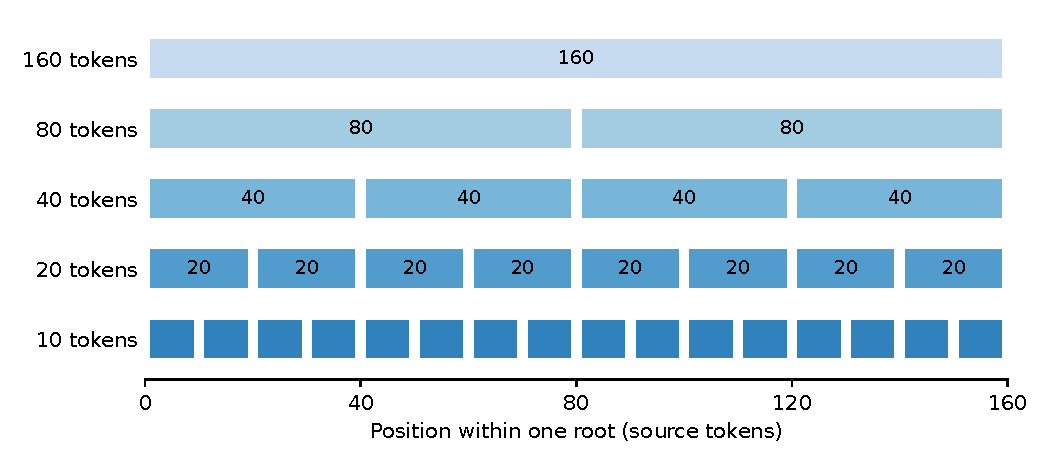
\includegraphics[width=\textwidth]{images/generated/tree_structure.pdf}
\caption{Aligned token spans within one complete 160-token root. Each
box is literal source text at a different scale. The illustration
shows containment, not measured relevance scores.}
\label{fig:tree}
\end{figure}

The level representation contains 85 features describing score
distributions separately at the five granularities. It includes summary
statistics, quantiles, concentration measures, softmax entropy, and
counts relative to score thresholds. The full tree representation adds
88 hierarchy-aware measurements for a total of 173. These include
parent--child gaps, sibling contrasts, and differences between adjacent
levels.

For example, a parent score minus the maximum child score describes
whether the coarse span matches the question better than its strongest
finer part. A mean child score measures a different property: whether
relevance is spread across the parent's descendants. Aggregating these
measurements across the paper gives a fixed-dimensional vector even
when papers have different numbers of chunks. The feature schema in
the repository defines the exact ordering and formulas.

The features use question-to-chunk similarity, not gold-evidence
similarity. Raw chunk embeddings are used to calculate scores but are
not concatenated as thousands of extra classifier inputs. A comparison
between stored/search scores and manually calculated cosine values
recorded a maximum absolute discrepancy of approximately
$1.09\times10^{-7}$, below the $10^{-5}$ audit tolerance.

\subsection{Linear and boosted-tree classifiers}
Phase 3A fits both level-only and full-tree linear classifiers. Five
paper-grouped training folds use seed 42. Nine candidates combine
learning rates 0.03, 0.01, and 0.003 with weight decays 0, 0.001, and
0.01. Each uses 300 full-batch epochs, training-fold standardisation,
and uniform cross-entropy. The hierarchy-based model is designated
the primary representation rather than chosen because of a favourable
validation result.

Phase 3B keeps those representations and replaces the linear classifier
with XGBoost. The grid combines maximum depths 2, 3, and 4; learning
rates 0.03 and 0.05; and 200 or 400 trees, giving 12 candidates per
representation. Other settings include minimum child weight 5,
row and column subsampling 0.8, L2 regularisation 1, and L1
regularisation 0. Square-root inverse-frequency weights address
class imbalance. Selection uses the grouped training folds, and the
tree model remains the primary method.

Simple score heuristics are also retained: maximum similarity,
top-five mean similarity, a training-tuned penalised top-five score,
and a leaf-breadth rule. Their purpose is to test whether broad
patterns are already captured by inexpensive hand-designed decisions.
Their reported classification results are not silently converted into
retrieval results where no corresponding evaluation was saved.

\section{Fusing language and similarity information}
\subsection{The initial fusion experiment}
Phase 3C combines a frozen Phase 2D classifier's five logits with the
173 tree features, producing 178 inputs to an XGBoost classifier.
An exploratory alternative concatenates its 1,024-dimensional hidden
representation with the same tree features, producing 1,197 inputs.
The primary logits-based variant is selected using training-fold
diagnostics.

There is an important weakness in this first procedure. The base Qwen
checkpoint has already been trained on all training questions. Its
features for those same questions are therefore in-sample features.
Dividing those rows into folds for the fusion classifier does not
undo that fact. The second-stage validation fold still contains
predictions produced by a base model that saw its labels during
training. The fusion cross-validation estimate is consequently
optimistic as an estimate of a fully unseen stacked pipeline.

The external validation predictions are not training rows for that
base fit, but the base checkpoint itself was selected using validation.
The original fusion result is retained as a development experiment
with these limitations, not presented as a clean final evaluation.

\subsection{Paper-grouped out-of-fold reconstruction}
Phase 3C-OOF reconstructs the language features correctly for the
meta-learner's training rows. For each of five paper-grouped folds,
Qwen is trained only on the other four folds and predicts the held-out
questions at a fixed third epoch. The fold sizes are 449, 449, 449,
450, and 448. Every training question receives a five-logit vector
from a model that did not train on that question's paper.

\begin{algorithm}[tbp]
\caption{Construction of out-of-fold language features}
\label{alg:oof}
\begin{algorithmic}[1]
\Require Training papers partitioned into folds $D_1,\ldots,D_5$
\For{$k=1,\ldots,5$}
  \State Train base router $f^{(-k)}$ on all papers outside $D_k$
  \State Use the fixed third-epoch checkpoint
  \For{question $q$ belonging to a paper in $D_k$}
    \State Store $\mathbf{z}^{\mathrm{OOF}}_q=f^{(-k)}(q)$
  \EndFor
\EndFor
\State Fit meta-model on $[\mathbf{z}^{\mathrm{OOF}}_q;\mathbf{x}^{\mathrm{tree}}_q]$
\State Refit the base router on all training papers for fixed three epochs
\State Predict validation logits with the refitted base router
\State Apply the meta-model to validation logits and tree features
\end{algorithmic}
\end{algorithm}

The full-data refit reproduces the fixed Phase 2D model state under the
recorded hash check. The fusion XGBoost configuration is inherited
and fixed at depth 2, learning rate 0.05, and 200 trees; this rerun does
not introduce another validation-tuned grid.

Out-of-fold construction fixes the in-sample base-feature problem.
It does not make every subsequent diagnostic fully nested: additional
meta-level cross-validation can still have dependencies through how
the base folds were constructed. Those diagnostics are not treated
as an unbiased nested estimate. Nor does this correction erase the
history of repeated external validation use.

\section{Expected-regret learning}
\label{sec:regret}
Phase 4 changes the question from \enquote{Which evidence-length class
is correct?} to \enquote{How much retrieval quality is lost by choosing
each size?} For every training question and size, define
\begin{equation}
C(q,g)=U^*(q)-U(q,g)\geq 0.
\label{eq:regret}
\end{equation}
Five XGBoost regressors predict these costs from the same 178-dimensional
combination of clean OOF Qwen logits and tree features. Each regressor
uses squared-error training, with the inherited fixed configuration
and no new hyperparameter search.

The routing rule is
\begin{equation}
\hat g(q)=\underset{g\in\granularities}{\arg\min}\,
\widehat C(q,g),
\label{eq:regretrule}
\end{equation}
with deterministic smaller-size tie-breaking. Since $U^*(q)$ is the
same for all candidate actions on a question, minimising true regret
is equivalent to maximising true retrieval utility. Under ideal
conditional-mean estimation, the same equivalence holds for expected
utility. In a finite fitted model, that reasoning motivates the
objective but does not guarantee that the selected action is optimal.

This formulation preserves information discarded by a single hard
label. Choosing a size whose F1 is almost maximal should incur a
small target cost even if it loses the argmax tie. Choosing a size
with much lower F1 should incur a larger cost. The regressors can
therefore learn useful distinctions between mistakes.

All 2,245 training utility vectors are complete in the final artifact.
Validation predictions are saved and hashed before the validation
utilities are read for scoring. Evaluation selects the corresponding
outcome from the five frozen actions rather than rerunning live
retrieval. This controls changes in the retrieval service and makes
the comparison an evaluation of the routing decision itself.

\section{Local tree-level routing}
\subsection{Changing the decision unit}
Phase 5A allows one paper to use several granularities for the same
question. The router is trained on the 4,081 gold-overlapping
question--tree pairs constructed in Chapter~\ref{ch:data}. Its
173-dimensional features have the same conceptual families as the
global tree representation but are computed within each local root.
The targets are local gold-overlap length categories.

The training class counts are $(557,876,1307,958,383)$ for the five
sizes. The XGBoost classifier inherits the fixed Phase 3B tree
configuration. Five paper-grouped folds provide diagnostics without
searching a new hyperparameter grid. No Qwen features are used in
this phase.

\subsection{Ranking trees and selecting chunks}
Trees are ranked independently of the predicted size. The score of
tree $T$ is an equal-weight average of its level-wise mean similarities:
\begin{equation}
S(q,T)=\frac{1}{|\granularities|}
\sum_{g\in\granularities}
\frac{1}{|\mathcal{C}_g(T)|}
\sum_{c\in\mathcal{C}_g(T)}s(q,c),
\label{eq:treescore}
\end{equation}
using available descendants and the implementation's handling of
partial edge trees. Equal weighting of levels prevents the sixteen
10-token leaves from dominating solely because they are more numerous.
It does not prove that the score is an optimal relevance estimator.

The five highest-ranked roots are retained. Within each root, the
classifier predicts a size and the single most similar chunk at that
size is returned. The primary output therefore contains five chunks,
potentially of different lengths. The router does not inspect gold
overlap to select validation trees.

The matched baseline uses exactly the same tree ranking, top-five
roots, and one-chunk-per-tree rule, but fixes the size to 40.
Additional fixed sizes are evaluated in the same way. This comparison
isolates the local size decision more directly than comparison with
global fixed-40 retrieval, which can select several chunks from one
root.

An exploratory variant returns all descendants at the predicted level
within each selected root. That variant changes the output budget
and is reported separately. Its additional evidence coverage cannot
be credited to a better five-chunk decision.

\section{A frozen context-need feature}
\subsection{Free generation and the validity gate}
Phase 5B asks whether a cheap semantic summary of the question can
help the local router. The frozen post-trained Qwen model predicts
one of three context-need categories: short, medium, or long. The
category is one-hot encoded and appended to each local tree feature
vector for that question, increasing the dimension from 173 to 176.
The language model is not fine-tuned on the local labels.

The first version uses deterministic free generation with a limit of
eight new tokens. It produces invalid responses on part of both splits,
including answers to the question instead of a category. The pipeline's
gate forbids replacing those failures with an arbitrary default and
proceeding as if the input feature were valid. No downstream classifier
result is claimed for that version.

\subsection{Constrained first-token scoring}
The repaired version first tests revised wording on the 175 previously
invalid training questions. It then uses a stronger output contract:
compare only the next-token logits for the verified single tokens
\texttt{short}, \texttt{medium}, and \texttt{long}, whose IDs are 8412,
25252, and 4670. One forward pass and an argmax produce a category;
there is no free text to parse.

The revised prompt explicitly tells the model not to answer the
question and to provide one lowercase label only. The full wording
is recorded in Appendix~\ref{app:protocols}. The training-only prompt
probe and final constrained evaluation are different operations:
the former tests wording on known training failures, while the latter
enforces validity for all required feature rows.

The local training examples, labels, tree ranking, and boosted-tree
protocol remain unchanged. The language model is frozen and receives
no task-label updates, so an OOF fine-tuning procedure is not required
to remove supervised in-sample predictions from this particular
feature. The experiment still shares the broader development-set
limitations of the rest of the thesis.

\section{What is held constant, and what is not}
Some comparisons isolate one change, such as the Phase 2C/2D prompt
or the Phase 5A/5B-v2 feature addition. Others redesign several
components, including the move from numeric generation to aliases
and from global to local routing. The results therefore distinguish
controlled effects from descriptive cross-phase differences.

\chapter{Evaluation, Results, and Discussion}
\label{ch:results}

\section{Evaluation protocol}
\subsection{Primary and secondary outcomes}
The main question-level comparison uses 924 validation questions and
paper-restricted top-five retrieval. Mean joined retrieval F1 is the
primary outcome; median F1 and mean regret provide complementary
descriptions. All five fixed-size outcomes are available for each
question, making the expected-regret comparison a paired choice among
the same saved actions.

Classification accuracy, macro F1, weighted F1, balanced accuracy,
and top-two accuracy describe the routing targets. Macro F1 gives
each class equal weight, which is useful when the evidence-length
labels are imbalanced. Top-two accuracy is meaningful only when the
model exposes comparable class scores. It is not reported as if
available for unrestricted numeric generation.

The local experiments retain all 924 questions for retrieval, but
their secondary classification diagnostic has a different unit:
2,074 gold-overlapping validation trees from 889 eligible questions.
Those trees are not the same as the 4,620 top-ranked trees used to
construct the primary retrieval outputs. Confusing these denominators
would produce an incorrect interpretation of local classification
accuracy.

\subsection{Paired paper-cluster bootstrap}
The later comparisons use 10,000 bootstrap replicates with seed 42.
Each replicate samples 277 paper identifiers with replacement and
includes all questions belonging to each sampled paper. A paper
sampled twice contributes its questions twice. The replicate statistic
is the question-weighted mean score or paired score difference over
the resulting sample.

For two methods $A$ and $B$, the observed difference is
\begin{equation}
\widehat\Delta_{A-B}=
\frac{1}{N}\sum_{q=1}^{N}
\bigl[\retrievalf^{A}(q)-\retrievalf^{B}(q)\bigr].
\end{equation}
The 2.5th and 97.5th percentiles of the bootstrap differences form
the reported 95\% interval. The same resampled papers are used for
both methods in a pair. This preserves their within-question pairing
and the clustering of questions within papers.

These intervals condition on the saved fitted models and the observed
development sample. They do not include variance from retraining,
hyperparameter search, prompt development, or unobserved datasets.
An interval that includes zero does not prove equivalence, and an
interval that excludes zero does not remove selection bias from
repeated validation use.

\section{Fixed granularity and oracle headroom}
% Generated by scripts/generate_results.py; do not hand-edit.
\begin{table}[htbp]
\centering\small
\caption{Fixed-size top-five retrieval on 924 validation questions.}
\label{tab:fixedresults}
\begin{tabular}{@{}lrrrr@{}}
\toprule
Size / method & Mean F1 & Median F1 & Regret & 95\% interval\\
\midrule
10 & 0.2211 & 0.2074 & 0.1610 & [0.2138, 0.2286]\\
20 & 0.2887 & 0.2809 & 0.0933 & [0.2800, 0.2975]\\
40 & 0.3159 & 0.3092 & 0.0662 & [0.3058, 0.3260]\\
80 & 0.2857 & 0.2666 & 0.0963 & [0.2746, 0.2966]\\
160 & 0.2168 & 0.1838 & 0.1653 & [0.2063, 0.2271]\\
Offline oracle & 0.3821 & 0.3836 & 0.0000 & [0.3717, 0.3923]\\
\bottomrule
\end{tabular}
\par\smallskip\begin{minipage}{\textwidth}\footnotesize Intervals use the Phase 4 paper-cluster bootstrap: 277 papers, 10,000 replicates, seed 42. The oracle is not deployable.\end{minipage}
\end{table}


Table~\ref{tab:fixedresults} shows a clear intermediate optimum among
the five evaluated sizes. Fixed 40 achieves 0.3159 mean retrieval F1,
ahead of fixed 20 at 0.2887 and fixed 80 at 0.2857. The two extremes
are weaker, with fixed 10 at 0.2211 and fixed 160 at 0.2168.
Figure~\ref{fig:fixed} visualises the pattern together with the
offline oracle.

\begin{figure}[tbp]
\centering
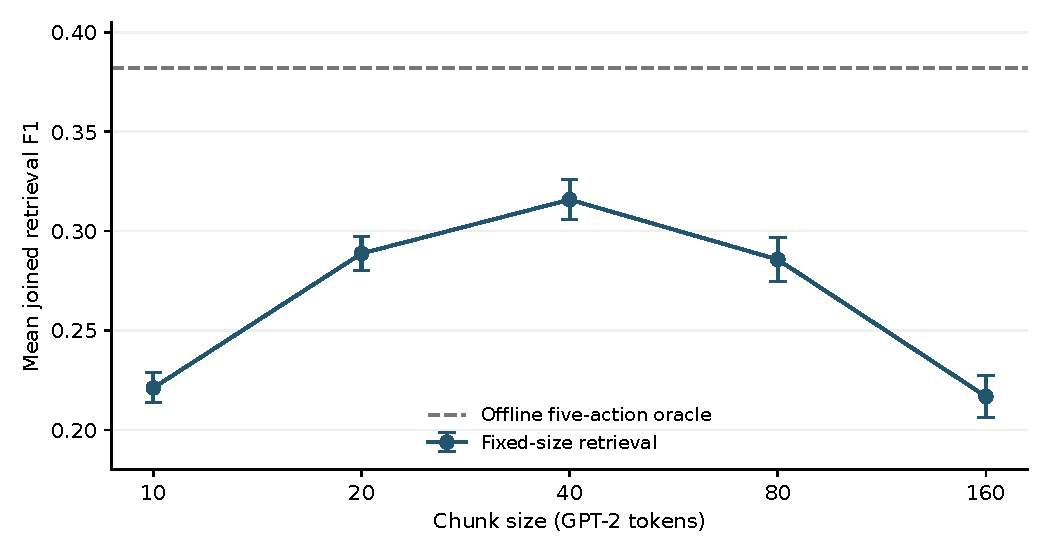
\includegraphics[width=\textwidth]{images/generated/fixed_granularity.pdf}
\caption{Fixed-size retrieval and the offline five-action oracle.
Error bars are 95\% paper-cluster bootstrap intervals for each fixed
method's mean, not intervals for all pairwise differences.}
\label{fig:fixed}
\end{figure}

The oracle reaches 0.3821, an absolute gain of 0.0662 over fixed 40.
Relative to the fixed-40 mean, this is approximately 21\% headroom.
The arithmetic describes the potential of selecting among the saved
actions; it does not predict how much of that potential a learner
can recover from observable features.

The exact retrieval-optimal size distribution includes every candidate:
138 questions prefer 10, 235 prefer 20, 282 prefer 40, 187 prefer 80,
and 82 prefer 160 under smaller-size tie-breaking. Thus fixed 40 is
the best aggregate setting without being the best action for most
individual questions. This is the strongest motivation for learning
an adaptive decision, and also a warning that the identity of the
best action can be difficult to predict.

The score diagnostics reveal a related tension. Mean query similarity
decreases from approximately 0.5490 at 10 tokens to 0.4271 at 160
tokens. Mean evidence similarity moves in the opposite direction,
from approximately 0.4538 to 0.5733. Joined retrieval F1 peaks between
the extremes. A router that simply maximises one similarity summary
therefore has no guarantee of optimising the primary metric.

\section{Early embedding and mixed-size experiments}
\subsection{Logistic regression versus the MLP}
The embedding router's logistic model achieves 0.2478 classification
accuracy and 0.2149 macro F1 against the legacy retrieval-derived
target. The MLP raises these to 0.2749 and 0.2187. Its macro-F1 gain
is only 0.0038, below the recorded 0.01 threshold for adopting the
more complex model.

The selected logistic router predicts counts
$(171,260,298,164,31)$ across the five sizes and reaches 0.2853
retrieval F1. It does not exceed fixed 40. The training-majority
legacy label is itself 40, and that constant reaches 0.3063
classification accuracy on validation, higher than either learned
classifier. Its macro F1 is much lower, 0.0938, because it predicts
only one class.

This comparison shows why no single classification summary tells
the full story. The learned model recognises more than one class,
but its errors cost enough retrieval quality to lose to a constant
size. The saved MLP result is a classification comparison only;
there is no full MLP retrieval score in the final baseline report.

\subsection{Raw and deduplicated mixtures}
Raw mixed-size retrieval reaches 0.2562 mean F1. Deduplication improves
it to 0.2618, but both remain below the selected embedding router
and the strongest fixed settings. The absolute deduplication gain
is approximately 0.0056.

\begin{table}[tbp]
\centering
\caption{Early adaptive baselines. The learned router uses the legacy
retrieval-derived label, not the later evidence-length target.}
\label{tab:early}
\begin{tabular}{@{}lrr@{}}
\toprule
Method & Mean retrieval F1 & Mean regret\\
\midrule
Question-embedding logistic router & 0.2853 & 0.0968\\
Mixed sizes, raw & 0.2562 & 0.1259\\
Mixed sizes, deduplicated & 0.2618 & 0.1203\\
\bottomrule
\end{tabular}
\end{table}

Of 4,620 raw mixed results, 2,708 are 10-token chunks and 1,148 are
20-token chunks. Together these account for more than 83\% of
returned chunks. Deduplication increases the 10-token count to
3,257, with 792 at 20 tokens. The procedure removes overlapping
spans after ranking; it does not recalibrate the ranking itself.
When a short candidate is ranked first, a larger containing passage
can subsequently be rejected.

The observed concentration on short chunks is consistent with the
cross-level query-score pattern. It is not sufficient to establish
that score scale is the only cause of mixed retrieval's lower F1.
Candidate counts, overlap, text boundaries, and the primary metric
also matter. The practical conclusion is narrower: raw pooling
and this overlap rule did not create a competitive adaptive baseline
in the evaluated setting.

\section{The question-only Qwen sequence}
% Generated by scripts/generate_results.py; do not hand-edit.
\begin{table}[htbp]
\centering\small
\caption{Question-only Qwen results on the evidence-length target.}
\label{tab:qwen_results}
\begin{tabular}{@{}llrrr@{}}
\toprule
Phase & Method & Accuracy & Macro F1 & Retrieval F1\\
\midrule
1 & Frozen Qwen & 0.0400 & 0.0490 & 0.2391\\
2 & Numeric SFT & 0.4318 & 0.1650 & 0.2266\\
2B-A & Uniform aliases & 0.3506 & 0.2092 & 0.2865\\
2B-B & Balanced aliases & 0.3701 & 0.1684 & 0.2496\\
2C & Base + class head & 0.3452 & 0.2176 & 0.2791\\
2D & Token-count prompt & 0.3690 & 0.2299 & 0.2767\\
2E & LR-grid winner & 0.3485 & 0.2278 & 0.2794\\
\bottomrule
\end{tabular}
\par\smallskip\begin{minipage}{\textwidth}\footnotesize Classification macro F1 and joined retrieval F1 measure different objectives.\end{minipage}
\end{table}


\subsection{Frozen prompting and numeric fine-tuning}
Phase 1 produces valid outputs for all 924 questions, but 767 predictions
are 10 tokens. Accuracy against evidence length is 0.0400 and macro
F1 is 0.0490. Its retrieval F1 is 0.2391. Valid formatting therefore
does not imply a useful decision.

Numeric fine-tuning changes the behaviour dramatically. The selected
Phase 2 checkpoint predicts 80 tokens 149 times and 160 tokens 775
times, never choosing the three smaller sizes. Accuracy rises to
0.4318 and macro F1 to 0.1650, while retrieval F1 falls to 0.2266.
Earlier checkpoints are even more concentrated on 160.

This is one of the clearest results in the thesis. The model has
become better at a proxy label while becoming worse at the evidence
retrieval task. Large evidence-length labels are common, particularly
in validation, but selecting five large chunks is a different action
from recovering that total evidence length. The result motivates a
change in supervision rather than an assumption that more training
alone will solve the mismatch.

For reference, a constant 80 prediction derived from the training
majority has validation accuracy 0.2511 and macro F1 0.0803. A
constant 160 prediction has validation accuracy 0.4545 and macro
F1 0.1250, but 160 is the validation majority rather than the
training majority. It is a descriptive comparison, not evidence
of a superior train-only baseline.

\subsection{Aliases and class balancing}
Uniform alias training in Phase 2B-A reaches macro F1 0.2092 and
retrieval F1 0.2865. It predicts 40 tokens 427 times, 80 tokens
189 times, and 160 tokens 308 times. This is a much less extreme
large-size distribution than numeric SFT, although the two smallest
classes remain unused.

Class-balanced alias training does not recover those missing classes.
Its selected second-epoch checkpoint predicts only 80 and 160, with
counts 434 and 490. Accuracy is slightly higher than in the uniform
variant, but macro F1 falls to 0.1684 and retrieval F1 to 0.2496.
Its top-two accuracy of 0.7056 exceeds the uniform variant's 0.6071,
which again does not make its top-one retrieval action better.

The controlled A/B experiment therefore gives no support for this
specific effective-number weighting scheme as an improvement. That
does not invalidate class weighting in general. The observed result
depends on a small, imbalanced dataset, the particular alias
formulation, a single recorded seed, and validation-selected
checkpoints.

\subsection{Classification head and explicit token counts}
The base-model classification head in Phase 2C reaches macro F1
0.2176 and retrieval F1 0.2791. It makes 20 predictions at size
20, but none at size 10. Its output distribution is less collapsed
than numeric SFT while still favouring medium and large sizes.

Changing only the instruction to explicit token counts in Phase 2D
raises accuracy from 0.3452 to 0.3690 and macro F1 from 0.2176
to 0.2299. Retrieval F1 moves in the opposite direction, from
0.2791 to 0.2767. Because neither prompt is truncated, the result
is not explained by the longer instruction removing question text.
The comparison supports an improvement in this classifier's label
prediction, not an improvement in the retrieval objective.

\subsection{Longer training and a learning-rate grid}
The Phase 2E winner, learning rate $5\times10^{-6}$ at epoch four,
achieves macro F1 0.2278 and retrieval F1 0.2794. It does not
exceed Phase 2D's macro F1, despite testing three learning rates
and fifteen epoch candidates. The best macro F1 in the other two
trials is approximately 0.2154 at $10^{-5}$ and 0.2252 at
$2\times10^{-5}$.

The small retrieval increase over Phase 2D is descriptive because
selection remains based on the repeatedly observed validation
classification metric. Only the selected global winner was evaluated
for final retrieval. The grid does not establish that longer
training is generally beneficial, nor that every checkpoint with
lower macro F1 would have lower retrieval F1.

\section{Similarity structure and feature fusion}
% Generated by scripts/generate_results.py; do not hand-edit.
\begin{table}[htbp]
\centering\small
\caption{Global similarity-tree and fusion results on the evidence-length target.}
\label{tab:tree_results}
\begin{tabular}{@{}llrrr@{}}
\toprule
Phase & Method & Accuracy & Macro F1 & Retrieval F1\\
\midrule
3A & Linear tree router & 0.3030 & 0.1928 & 0.2677\\
3B & XGBoost tree router & 0.3290 & 0.2247 & 0.2717\\
3C & Original fusion & 0.3193 & 0.2307 & 0.2872\\
3C-OOF & Corrected fusion & 0.3225 & 0.2100 & 0.2783\\
\bottomrule
\end{tabular}
\par\smallskip\begin{minipage}{\textwidth}\footnotesize Classification macro F1 and joined retrieval F1 measure different objectives. Original fusion has in-sample base-feature contamination in its training-fold evaluation.\end{minipage}
\end{table}


\subsection{From linear score features to boosted trees}
The Phase 3A full-tree linear model reaches validation macro F1
0.1928 and retrieval F1 0.2677. Its level-only counterpart has
macro F1 0.1892. The difference is small, and the selected
level-only model has slightly higher training OOF macro F1 than
the selected tree model, approximately 0.2253 versus 0.2222.
There is no consistent large hierarchy gain in this linear setup.

The heuristic diagnostics are also limited. Maximum similarity and
top-five mean similarity have validation macro F1 of 0.0600 and
0.0573. The training-tuned penalised score reaches 0.1434, while
the leaf-breadth rule reaches 0.1242. The latter's accuracy is
0.3755, illustrating again how a comparatively favourable accuracy
can coexist with weak class-balanced performance.

XGBoost improves the primary full-tree result in Phase 3B to
macro F1 0.2247 and retrieval F1 0.2717. The retrieval increase
over the linear tree model is about 0.0040. The level-only
XGBoost model has validation macro F1 0.1822. Nonlinear use of
the full representation is more promising than the particular
linear model, but the retrieval outcome is still below fixed
20, fixed 40, and the strongest question-only alias variant.

Score features therefore contain some usable information without
making the evidence-length proxy an effective retrieval objective.
The results should not be read as proving that a literal hierarchy
is intrinsically superior to all flat representations; the models,
feature definitions, and small hyperparameter grids define the
scope of that comparison.

\subsection{Original fusion and its corrected rerun}
Original Phase 3C fusion reaches macro F1 0.2307 and retrieval F1
0.2872. These are improvements over the primary Phase 3B result.
However, the training-fold fusion estimate uses in-sample Qwen
features, as explained in Chapter~\ref{ch:method}.

The exploratory hidden-state fusion has validation accuracy 0.3203
and macro F1 0.2298, close to the logits variant. Its training-fold
macro F1 is 0.3544, below the logits variant's 0.3838, so the
compact logits representation is retained. The hidden-state variant
does not have the primary final retrieval evaluation.

The corrected OOF experiment reduces the apparent training-fold
macro F1 from approximately 0.3838 to 0.2317, and accuracy from
0.4717 to 0.3042. The external validation result is macro F1
0.2100 and retrieval F1 0.2783, below the original fusion by
approximately 0.0089 retrieval F1.

It would be misleading to describe this only as a failed attempt to
improve a score. The corrected training interface answers a more
credible question. Its lower result indicates that the earlier
optimism cannot be carried forward unchanged. The rerun preserves
the useful idea of combining signals while removing an identifiable
source of training contamination.

\begin{figure}[tbp]
\centering
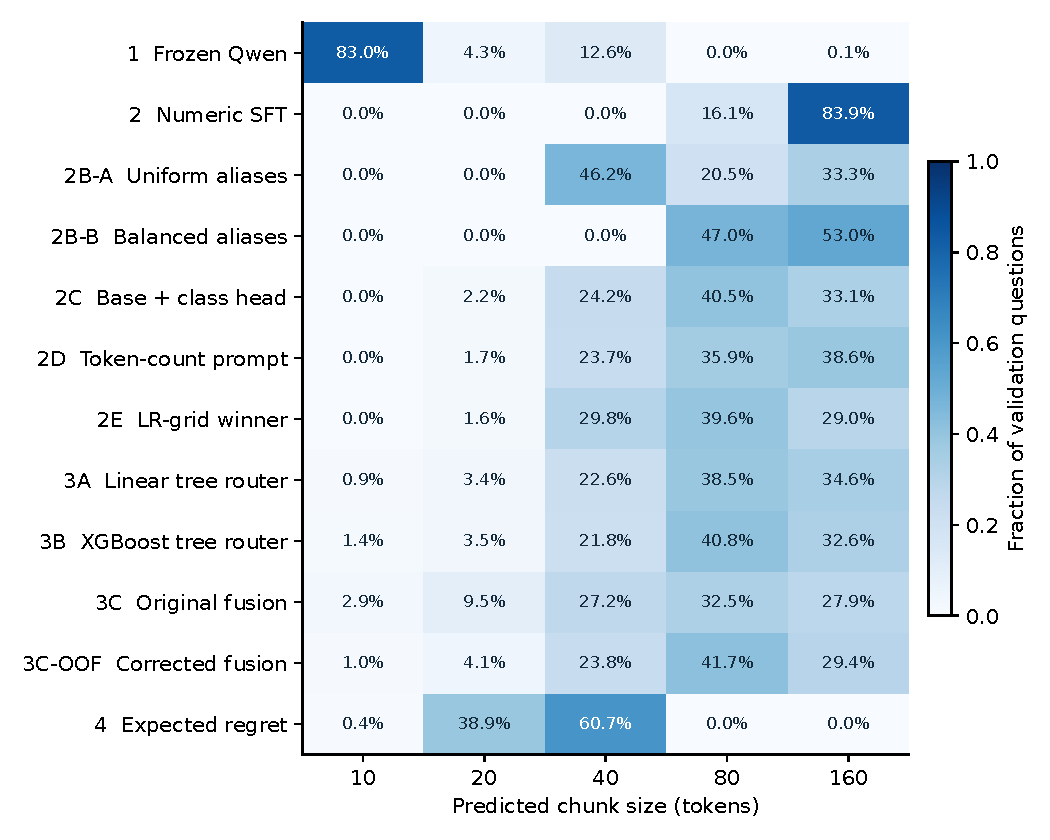
\includegraphics[width=\textwidth]{images/generated/prediction_heatmap.pdf}
\caption{Predicted granularity distributions across the main
question-level phases. Rows sum to 100\%. Phase 4 optimises retrieval
regret; the preceding rows use evidence-length classification.}
\label{fig:predictions}
\end{figure}

Figure~\ref{fig:predictions} shows why aggregate label metrics need
the accompanying prediction distributions. Most evidence-length
classifiers assign many questions to 80 or 160. The expected-regret
router discussed next behaves differently even though it uses
the same families of observable features as corrected fusion.

\section{Expected regret: the strongest learned global router}
Phase 4 reaches mean retrieval F1 0.3075 and median F1 0.3008.
Its mean regret is 0.0746. It chooses 10 tokens for four questions,
20 for 359, and 40 for 561; it never selects 80 or 160 on validation.
Compared with the preceding evidence-length models, the decision
distribution shifts strongly towards the sizes that perform well
under joined retrieval F1.

% Generated by scripts/generate_results.py; do not hand-edit.
\begin{table}[htbp]
\centering\small
\caption{Expected-regret router (Phase 4) minus each comparator.}
\label{tab:pairedregret}
\begin{tabular}{@{}lrr@{}}
\toprule
Comparator & Mean F1 difference & 95\% interval\\
\midrule
2D & +0.03079 & [+0.02174, +0.04003]\\
3B & +0.03579 & [+0.02663, +0.04483]\\
Original 3C & +0.02030 & [+0.01162, +0.02877]\\
3C-OOF & +0.02920 & [+0.01987, +0.03864]\\
Fixed 40 & -0.00835 & [-0.01266, -0.00416]\\
\bottomrule
\end{tabular}
\par\smallskip\begin{minipage}{\textwidth}\footnotesize Paired paper-cluster bootstrap with 10,000 replicates and seed 42. Positive values favour Phase 4.\end{minipage}
\end{table}


The paired comparisons in Table~\ref{tab:pairedregret} favour Phase 4
over Phase 2D, Phase 3B, original fusion, and corrected fusion.
The respective mean gains are 0.0308, 0.0358, 0.0203, and 0.0292.
Their paper-cluster intervals exclude zero in the observed development
sample. These results support the practical value of aligning the
training target with retrieval utility.

\begin{figure}[tbp]
\centering
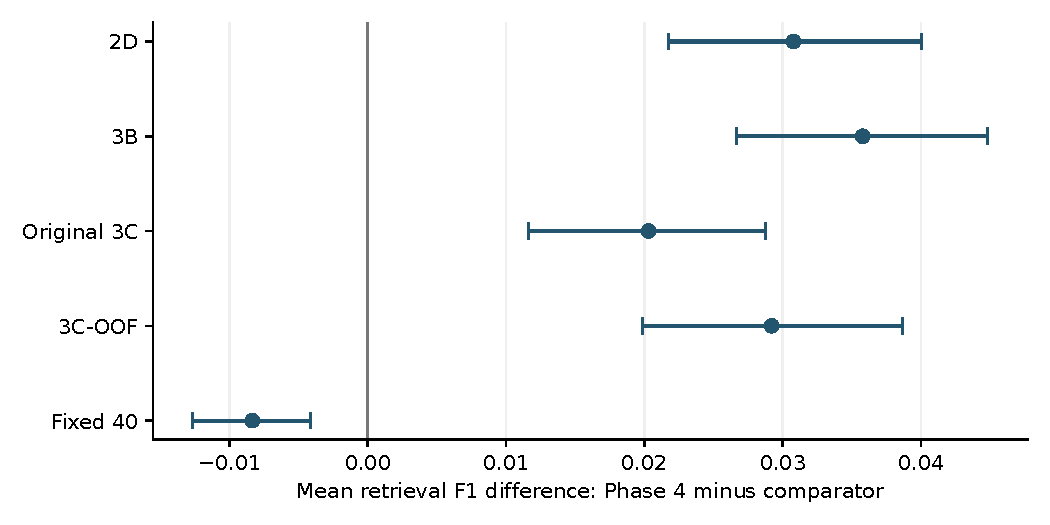
\includegraphics[width=\textwidth]{images/generated/regret_differences.pdf}
\caption{Paired mean retrieval-F1 differences for Phase 4. Intervals
are obtained by resampling papers, not by retraining the models.}
\label{fig:regret}
\end{figure}

The main baseline remains stronger. Phase 4 minus fixed 40 is
$-0.00835$, with interval $[-0.01266,-0.00416]$. Consequently,
the strongest learned question-level router in the repository does
not establish an advantage over fixed 40. It narrows the gap left
by the earlier learned methods without closing it.

The fraction of questions with zero regret is 280/924, or 0.3030.
This allows any equally optimal action. Accuracy against an exact
smaller-tie label is slightly different, 0.3019. Neither should
be substituted for the other. Against the evidence-length labels,
Phase 4 has accuracy only 0.1418 and macro F1 approximately 0.1060.
That low proxy score is entirely compatible with its stronger
retrieval outcome.

The absence of large-size predictions is also a limitation. The
oracle still prefers 80 or 160 for many questions. The model
appears to learn a useful conservative preference without reliably
identifying those exceptions. A good average action is not the
same as a successful instance-level explanation of evidence need.

\section{Three concrete routing cases}
The following cases are drawn directly from the frozen validation
records, with the original question wording retained. The first is
the largest Phase 4 gain over fixed 40, the second the largest loss,
and the third illustrates a near tie. They are deliberately selected
diagnostics, not a random sample or an estimate of how often each
pattern occurs.

% Generated, deliberately selected diagnostic cases; not a random sample.
\par\medskip\noindent\begin{minipage}{\textwidth}
\textbf{Case 1: Did they collect their own datasets?}\par\smallskip
Paper 1608.01884. Phase 4 selects 10 tokens. The F1 difference from fixed 40 is $+0.277200$.
\begin{center}\small\begin{tabular}{@{}lrrrrr@{}}\toprule
Size & 10 & 20 & 40 & 80 & 160\\\midrule
Retrieval F1 & 0.5432 & 0.3103 & 0.2660 & 0.1552 & 0.1291\\
\bottomrule\end{tabular}\end{center}
\end{minipage}\par\medskip

\par\medskip\noindent\begin{minipage}{\textwidth}
\textbf{Case 2: Did they used dataset from another domain for evaluation?}\par\smallskip
Paper 1909.03582. Phase 4 selects 20 tokens. The F1 difference from fixed 40 is $-0.322390$.
\begin{center}\small\begin{tabular}{@{}lrrrrr@{}}\toprule
Size & 10 & 20 & 40 & 80 & 160\\\midrule
Retrieval F1 & 0.2357 & 0.3032 & 0.6256 & 0.8213 & 0.5610\\
\bottomrule\end{tabular}\end{center}
\end{minipage}\par\medskip

\par\medskip\noindent\begin{minipage}{\textwidth}
\textbf{Case 3: What experiments are conducted?}\par\smallskip
Paper 1909.06200. Phase 4 selects 20 tokens. The F1 difference from fixed 40 is $+0.003092$.
\begin{center}\small\begin{tabular}{@{}lrrrrr@{}}\toprule
Size & 10 & 20 & 40 & 80 & 160\\\midrule
Retrieval F1 & 0.1750 & 0.3636 & 0.3605 & 0.3097 & 0.1997\\
\bottomrule\end{tabular}\end{center}
\end{minipage}\par\medskip


In the first case, a rare 10-token decision is useful: its F1 is
0.5432, above all four larger alternatives. This demonstrates that
the router is not simply a disguised constant-40 method. In the
second case, the 20-token decision misses a substantial opportunity:
80-token retrieval reaches 0.8213 while the chosen action reaches
0.3032. The question's short wording alone does not justify a
short evidence window.

The third case explains why a cost-sensitive target can be more
informative than a hard class. Choosing 40 instead of the optimal
20 would lose only about 0.0031 F1. A classification metric marks
that decision wrong, just as it marks a much more damaging choice
wrong. Regret preserves the difference in severity.

These examples describe observed utility patterns. They do not
show that any model generated a correct answer, and they do not
establish the semantic sufficiency of the retrieved chunks without
separate evidence inspection.

\section{Local tree-level retrieval}
% Generated by scripts/generate_results.py; do not hand-edit.
\begin{table}[htbp]
\centering\small
\caption{Matched local retrieval: five ranked trees, one chunk per tree.}
\label{tab:localresults}
\begin{tabular}{@{}lrrrr@{}}
\toprule
Method & Precision & Recall & F1 & Tokens\\
\midrule
Same-tree fixed 10 & 0.3829 & 0.1932 & 0.2195 & 53.8\\
Same-tree fixed 20 & 0.3440 & 0.3237 & 0.2820 & 103.6\\
Same-tree fixed 40 & 0.2846 & 0.4862 & 0.3075 & 202.7\\
Same-tree fixed 80 & 0.2103 & 0.6469 & 0.2791 & 400.5\\
Same-tree fixed 160 & 0.1385 & 0.7833 & 0.2135 & 792.5\\
Phase 5A local & 0.2754 & 0.5114 & 0.3053 & 232.8\\
Phase 5B-v2 & 0.2739 & 0.5120 & 0.3045 & 234.8\\
\bottomrule
\end{tabular}
\par\smallskip\begin{minipage}{\textwidth}\footnotesize Each score is a mean over 924 questions. Tokens are measured in the saved retrieval output, not inferred from nominal chunk size.\end{minipage}
\end{table}


Phase 5A returns one chunk from each of five selected trees and
achieves mean precision 0.2754, recall 0.5114, and F1 0.3053.
The matched same-tree fixed-40 method reaches precision 0.2846,
recall 0.4862, and F1 0.3075. Local adaptation gains some recall
but loses enough precision that its F1 is slightly lower.

The paired difference is $-0.00220$, with a 95\% paper-cluster
interval of $[-0.00580,0.00145]$. The observed difference does
not demonstrate a local-routing advantage. The interval also does
not establish that the two methods are equivalent; an equivalence
claim would need an explicit margin and an appropriate test.

Phase 5A makes 4,620 local size predictions, with counts
$(246,529,2823,965,57)$. Forty tokens dominates, which is consistent
with its role as a strong local default. The mean retrieved token
count is 232.8, compared with 202.7 for the same-tree fixed-40
method. Equal chunk counts therefore still leave a difference
in text budget.

The secondary gold-overlap classification diagnostic has accuracy
0.2850 and macro F1 0.2144. It helps assess the local target but
does not evaluate how well the method selected the five trees:
those diagnostic examples are constructed using gold overlap,
whereas inference ranks all available trees without gold.

Returning all chunks at the predicted level changes the outcome
substantially. Mean recall rises to 0.7826, but precision falls to
0.1382 and F1 to 0.2131. The method now returns an average of
22.44 chunks and 809.5 tokens. This exploratory result demonstrates
the cost of indiscriminate coverage within selected regions, not
an improvement under the primary top-five budget.

Global fixed 40 and same-tree fixed 40 must remain separate.
Their F1 values are 0.3159 and 0.3075, respectively. Requiring
one chunk per root imposes spatial diversity and can exclude
multiple useful chunks from one region. The matched local baseline
is therefore essential for isolating the router's contribution.

\section{The final Qwen context-feature experiment}
\subsection{An invalid-output failure that was not hidden}
The first Phase 5B version produces 175 invalid outputs among
2,101 eligible training questions and 56 among 924 validation
questions. There are 231 invalid outputs in total. Among valid
training categories, the counts are 54 short, 1,867 medium, and
five long; validation has 31 short, 836 medium, and one long.

Some outputs answer the underlying question rather than estimate
context need. A default category would hide that interface failure.
The pipeline instead stops before downstream classifier training.
This version has no final retrieval score and is not treated as
a completed ablation with poor performance.

\subsection{Valid constrained outputs, little additional information}
The training-only wording repair succeeds on 173 of the 175
previous failures under its probe. Two failures remain, motivating
the constrained first-token decision. The final Phase 5B-v2
feature has no invalid outputs, but its distribution is highly
concentrated: training has 24 short, 2,076 medium, and one long;
validation has 12 short, 912 medium, and no long.

Thus 98.70\% of validation questions receive the same category.
The feature is correctly formatted but has very little variation.
The resulting local router reaches retrieval F1 0.3045, compared
with 0.3053 for Phase 5A. The difference is $-0.00073$, with
interval $[-0.00236,0.00088]$. Against same-tree fixed 40, the
difference is $-0.00293$, with interval $[-0.00646,0.00069]$.
Neither comparison demonstrates an improvement.

The local prediction distribution changes slightly to
$(247,506,2804,1008,55)$, and secondary local classification
accuracy and macro F1 are approximately 0.2811 and 0.2123.
The added feature therefore changes the fitted decisions, but
not in a way supported as beneficial by the primary outcome.
Output validity and feature usefulness are separate requirements.

\section{Engineering and computational observations}
The repository records substantial work that does not correspond
to a new row of retrieval F1: ingestion retries, smoke tests,
tiny-overfit checks, accumulation-tail preflights, checkpoint
recovery, score audits, feature extraction resumption, and
pre-evaluation hash locks. Their role is to establish that the
reported row means what it claims to mean.

The corrected fusion procedure illustrates the additional training
cost of methodological care. The recorded total is about 7,712
seconds, or two hours and eight minutes, including five fold
fits, a full-data refit, feature extraction, meta-model fitting,
and retrieval evaluation. The five fold fits account for about
5,888 seconds and the refit for about 1,434 seconds. Maximum
recorded allocated GPU memory is approximately 9.03 GB, with
9.60 GB reserved.

These figures describe that recorded execution, not a general
latency benchmark. Earlier zero-shot generation, GPU fine-tuning,
CPU tree fitting, cached feature use, and live retrieval have
different hardware and timing boundaries. Comparing their wall
times as though they were interchangeable online requests would
be misleading.

At prediction time, a question-only router can choose a size
before retrieval. A similarity-tree router needs similarities
across the paper and all levels before deciding. Even if many
values are cached, that extra information has an acquisition
cost. The current study measures retrieval quality more completely
than end-to-end deployment efficiency. A future system should
report both the cost of feature construction and the cost of
the final returned context.

\section{Threats to validity}
\subsection{Repeated validation and limited random seeds}
The most important limitation is repeated validation use.
Checkpoint selection, prompts, representations, and subsequent
research directions were informed by this split over time.
Training-only decisions in later phases improve local experimental
discipline but do not erase that history. The thesis therefore
does not present the final numbers as untouched test performance.

Most main training results use one recorded seed. Bootstrap
intervals resample evaluation papers while holding fitted models
fixed; they do not quantify the variation across independent
training runs. The many development comparisons also create a
multiple-comparison context. Intervals are reported for specified
pairs without claiming a family-wide corrected discovery.

\subsection{Metric and budget validity}
Joined token F1 measures lexical agreement with annotated
evidence. It can penalise helpful explanatory context and reward
matching tokens that occur outside the annotated source span.
It does not evaluate factual correctness, entailment, citation
accuracy, or answer generation. Its values should not be
presented as a full RAG quality score.

The fixed-size comparisons hold the chunk count constant while
allowing the total text budget to vary. Local routing holds
the number of selected trees and returned chunks constant, but
still changes total length. The results identify useful settings
under those protocols; a constant-token-budget experiment could
lead to a different ranking.

\subsection{Data and representation validity}
The study uses scientific NLP papers, a single fixed embedding
model, a small discrete size set, and paper-restricted retrieval.
Sentence-aware chunks, contextual chunk embeddings, other
domains, corpus-level negatives, and different annotation
practices may change the behaviour.

The local target further depends on evidence that can be mapped
to text offsets. Partial mappings and excluded table/figure
evidence create a selection effect. The primary validation
retrieval includes all frozen questions, but the local classifier
learns from a narrower subset of evidence types.

\subsection{Causal interpretation}
The sequence contains both controlled ablations and broader
redesigns. A prompt-only change supports a narrower conclusion
than a change of model family, feature source, and target.
The thesis avoids treating every later phase as proof that
one named component caused a gain. The strongest defensible
interpretation is comparative: under the preserved configurations,
utility-aware learning improved the learned global decision,
while neither global nor local adaptation surpassed its
strong fixed-size reference.

\section{Synthesis}
Three lessons recur across the experimental history. First,
the target is decisive. Evidence length is interpretable but
does not directly describe the utility of five retrieved chunks.
Second, more information is useful only when it is both validly
constructed and informative: corrected OOF fusion reduces
optimism, while constrained Qwen outputs fix formatting without
creating category diversity. Third, a fixed baseline deserves
to remain in every comparison. Here it prevents a progression
of increasingly complex methods from being mistaken for a
progression of consistently better retrieval systems.

\chapter{Conclusion and Future Work}
\label{ch:conclusion}

\section{What the study found}
This thesis began with a reasonable expectation: questions that need
different amounts of evidence should benefit from different retrieval
granularities. The experiments support the premise that the best size
varies across questions, but they do not establish that the evaluated
routers can exploit that variation better than a strong fixed setting.

On the frozen validation set, fixed 40-token retrieval reaches mean
joined evidence-token F1 of 0.3159. The offline best-of-five oracle
reaches 0.3821, leaving a meaningful gap. The strongest learned
question-level method, expected-regret routing, reaches 0.3075.
Local tree-level routing reaches 0.3053, compared with 0.3075 for
its matched fixed-40 tree baseline. Adding a frozen Qwen
context-need feature does not demonstrate an improvement.

The sequence separates the promise of adaptation from the information
and supervision needed to turn it into a reliable decision.

\section{Answers to the research questions}
\subsection{RQ1: Is there headroom beyond a fixed size?}
Yes, within the five saved retrieval actions. The offline oracle
improves mean F1 by 0.0662 over fixed 40, and its selected sizes
cover the full candidate set. A single size is therefore not
optimal for every question. However, oracle headroom alone does
not show that the correct decision is predictable without access
to gold evidence. It establishes opportunity, not deployability.

\subsection{RQ2: Is the question alone sufficient?}
The evaluated question-only methods do not beat fixed 40.
The embedding router reaches 0.2853 retrieval F1, while the
strongest retrieval result among the reported Qwen question-only
variants is 0.2865 for uniform alias training. Fine-tuning and
classification-head changes improve some label metrics without
consistently improving retrieval.

The clearest counterexample is numeric SFT: label accuracy
increases from 0.0400 to 0.4318 relative to frozen prompting,
but retrieval F1 decreases. This shows that learning the
evidence-length category is not an adequate substitute for
learning a useful retrieval action in this protocol.

\subsection{RQ3: Does similarity structure help?}
Similarity-tree features provide additional observable information.
The weighted boosted-tree setup improves mean retrieval F1 and macro
F1 over the tested uniformly weighted linear tree model, but does not
isolate a benefit from nonlinearity alone. Original fusion looks promising,
but its in-sample base features make the training-fold estimate
optimistic. Corrected OOF fusion reaches 0.2783 retrieval F1.

The evidence therefore supports investigating combined language
and document signals, but not claiming that hierarchy or fusion
alone solves granularity selection. The corrected training
procedure is a methodological contribution even though it lowers
the apparent result.

\subsection{RQ4: Does retrieval-utility supervision help?}
Yes, relative to the preceding learned global methods in the
recorded development comparisons. Expected-regret learning
reaches 0.3075 F1, with positive paired differences over
Phase 2D, Phase 3B, and both fusion versions. The change of
objective also produces a markedly different prediction
distribution, concentrating on 20 and 40 rather than 80 and 160.

It still falls short of fixed 40 by 0.00835 F1. The result
supports objective alignment as a productive direction, not
a final superiority claim for the learned router.

\subsection{RQ5: Does local adaptation add value?}
The local protocol allows different regions to contribute
different chunk sizes, but the trained router does not demonstrate
an advantage over the same-tree fixed-40 baseline. Its slight
recall gain comes with lower precision. Returning all chunks
at each predicted level raises recall much further while
reducing F1 and substantially increasing the output budget.

The frozen Qwen context feature also adds no demonstrated gain.
Constrained scoring successfully removes invalid outputs, but
almost every question receives the category medium. A reliable
interface is necessary; it does not guarantee a discriminative
feature.

\section{Implications for adaptive retrieval}
The most useful design principle is to define the retrieval action
before its label. If the action returns five chunks, the target
should reflect their utility. Total annotation length is an
intuitive property, but it is not the action itself.

A second principle is to account for information cost. A question-only
router needs less preparation than one that inspects every level
of a paper. Additional features must earn their cost through a
measurable quality or efficiency benefit.

A third principle is to retain strong controls as the research
becomes more sophisticated. The global fixed-size baseline,
the matched local baseline, and the OOF reconstruction each
prevent a different misleading comparison. They are part of
the scientific result, not merely implementation details.

\section{Future work}
\subsection{Independent evaluation and repeated training}
The immediate priority is an untouched evaluation split with
a frozen protocol. The action set, target, feature extraction,
hyperparameters, checkpoint rule, and primary metric should
be fixed before inspecting its outcomes. Repeated training
seeds would then distinguish stable gains from a favourable
single fit.

If further model selection is required, it should occur inside
paper-grouped training procedures, with nested construction
for stacked models where appropriate. The external evaluation
should be used once for the specified comparison. Additional
datasets would test whether the observed preference for an
intermediate size is specific to QASPER and this metric.

\subsection{Utility-aware local decisions}
The most direct modelling extension is to bring the Phase 4
objective into the local setting. Instead of predicting local
evidence length, a tree-level learner could estimate the
incremental retrieval utility of each candidate chunk. This
would also expose an interaction that the current local
classifier ignores: a useful chunk may become redundant after
another tree has already contributed similar evidence.

A set-level decision under an explicit token budget would
address that interaction more naturally. Candidate selection
could stop when further text adds little expected evidence
coverage, rather than always returning five independent
decisions. This is a proposed experiment, not an implemented
result of the repository.

\subsection{Calibration and selective adaptation}
Most questions in Phase 4 are assigned 20 or 40, while some
large-size oracle opportunities are missed. A selective router
could use fixed 40 as a default and deviate only when the
predicted utility difference is sufficiently large and
well-calibrated. The threshold would need training-only
selection, and performance should be reported as a function
of both deviation frequency and retrieval cost.

The question is whether the system can identify when changing
a strong default is worthwhile. The current results motivate
that experiment without answering it.

\subsection{Representations, budgets, and generation}
Sentence-aware or proposition-based units could reduce the
boundary failures of short token windows. Contextual chunk
embeddings could preserve neighbouring information without
always returning longer passages. Both changes should be
evaluated with matched candidate and token budgets, since
otherwise a representation effect can be confused with an
increase in returned text.

A complete RAG evaluation should then test whether changes in
retrieved evidence improve generated answers. It should hold
the generator, prompt, context ordering, and generation
settings constant, and measure answer correctness, evidence
support, and citation quality alongside retrieval F1. Questions
requiring tables or figures deserve separate analysis rather
than exclusion from every stage.

Finally, a deployment-oriented study should measure indexing
cost, feature-extraction latency, model memory, retrieval
latency, and total supplied tokens under comparable hardware
conditions. An adaptive method can be useful by saving
resources at similar quality, even if its absolute F1 does
not exceed the best fixed baseline. That trade-off was not
established by the present experiments.

\section{Closing remarks}
Adaptation must earn its place against a strong fixed baseline.
Here, utility-aware supervision and cleaner evaluation made progress,
but did not establish superiority. The next step is to test that
direction on untouched data under a fixed protocol.

\appendix
\chapter{Experimental Chronology}
\label{app:chronology}
This appendix records the development sequence rather than presenting
only the final model. Phase names follow the repository. Infrastructure
checks and interrupted runs are identified separately from completed
retrieval evaluations.

\begin{center}
\small
\captionsetup{hypcap=false}
\captionof{table}{Chronology of the preserved experimental programme.}
\label{tab:chronology}
\begin{tabular}{@{}>{\raggedright\arraybackslash}p{2cm}>{\raggedright\arraybackslash}p{5.3cm}>{\raggedright\arraybackslash}p{5.8cm}@{}}
\toprule
Stage & Purpose & Outcome or status\\
\midrule
Initial prototype & Weaviate ingestion, JSON exports, sample retrieval & First working data path; no comparative vector-store benchmark\\
Foundation & Evidence filtering, parallel paper processing, Qdrant migration & Five chunk levels, resumable stages, stable identities\\
Early smoke & Verify retrieval and output writing & Tiny and empty artifacts are execution diagnostics, not full validation results\\
Integrity & Audit counts, offsets, checkpoints, and missing records & Dated problems documented; later frozen artifacts define final populations\\
Metric and storage & Per-chunk diagnostics, schema v2, configuration-aware identities & Persistence and idempotency checks; joined F1 remains primary\\
Fixed baseline & Score all five sizes, top five within each paper & Fixed 40 strongest; offline oracle records per-question opportunity\\
Embedding router & Logistic regression and 64-unit MLP & MLP gain below adoption threshold; logistic router retained\\
Mixed sizes & Pool candidates, with and without overlap removal & Neither raw nor deduplicated mixture beats fixed 40\\
Phase 1 & Frozen Qwen, question-only numeric decision & Valid outputs, strong preference for size 10\\
\bottomrule
\end{tabular}
\end{center}
\newpage
\begin{center}
\small
\textbf{Table~\ref{tab:chronology} (continued)}\par\medskip
\begin{tabular}{@{}>{\raggedright\arraybackslash}p{2cm}>{\raggedright\arraybackslash}p{5.3cm}>{\raggedright\arraybackslash}p{5.8cm}@{}}
\toprule
Stage & Purpose & Outcome or status\\
\midrule
Phase 2 preflights & Smoke, tiny-overfit and training-loop checks & Tail-accumulation issue corrected; interrupted v1 not a final model\\
Phase 2 v2 & Numeric supervised fine-tuning & Better label accuracy, weaker retrieval, large-size collapse\\
Phase 2B-A & Uniform restricted-alias classification & More medium-size predictions; strongest Qwen-only retrieval result\\
Phase 2B-B & Effective-number class weighting & No small-class recovery; weaker macro F1 and retrieval than A\\
Phase 2C & Base model with five-class head & Higher macro F1 than numeric SFT, but lower accuracy\\
Phase 2D & Exact token-count prompt & Better classification than 2C, slightly lower retrieval F1\\
Phase 2E & Three learning rates, five epochs & Fifteen candidates; winner 5e-6 at epoch four\\
Phase 3A & Level and hierarchy features with linear models & Small hierarchy difference; heuristics retained as diagnostics\\
Phase 3B & Weighted XGBoost on both representations & Training-fold macro F1 selects full tree; mean retrieval improves, median falls\\
Phase 3C & Qwen logits or hidden states fused with tree features & Initial result limited by in-sample base features\\
Phase 3C-OOF & Reconstruct base features using paper-grouped held-out predictions & Less optimistic fusion estimates; fixed full-data refit\\
Phase 4 & Five retrieval-regret regressors & Best learned global retrieval; still below fixed 40\\
Phase 5A & Gold-overlap supervision for local tree decisions & Close to, but not better than, matched fixed-40 tree retrieval\\
Phase 5A probe & Return all descendants at predicted level & Higher recall, larger budget, much lower F1\\
Phase 5B v1 & Frozen Qwen context category from free generation & Invalid-output gate fails; no downstream result\\
Phase 5B-v2 & Training-only prompt repair and constrained token scoring & Valid but nearly constant feature; no demonstrated retrieval gain\\
\bottomrule
\end{tabular}
\end{center}

Preflight runs check gradients, tiny-set fitting, accumulation, and
recovery; they are not independent estimates of generalisation.
Source transfers and hash audits likewise preserve an experiment
rather than create a new model. Phase 3A resumed gRPC feature
extraction through REST after 1,844 training questions. Its durable
processing-time sum must not be mistaken for uninterrupted wall time.

\chapter{Configurations and Output Contracts}
\label{app:protocols}

\section{Common retrieval settings}
The common settings are the candidate sizes 10, 20, 40, 80, and 160;
GPT-2 tokenisation; fixed 1,536-dimensional
\texttt{text-embedding-3-small} vectors; cosine similarity; source-paper
filtering; and top-five retrieval for the primary protocols.
The metric configuration hash preserved in the main frozen comparisons is
\begin{quote}\small
\path{9a3022fd1c808f72ccbf3265fe6020593bb58bdd28aeb9025b8c4b735d669de8}.
\end{quote}
The metric name is \texttt{f1\_joined\_topk}; the metric version is
\texttt{qasper-token-prf-v2}. A change in normalisation, candidate
population, or top-$K$ is a new evaluation configuration.

The three target definitions are
\begin{itemize}
\item \path{oracle-f1-evidence-smaller-v1}: legacy retrieval-derived labels;
\item \path{oracle-evidence-length-gpt2-smaller-midpoint-v1}: total evidence length;
\item local gold-overlap labels constructed for question--tree pairs.
\end{itemize}
The last target is described by its construction in
Chapter~\ref{ch:data}; it must not be assumed identical to a global
label merely because both return one of the same five numbers.

\section{Model identities and training}
The post-trained Qwen model is pinned to revision
\begin{quote}\small
\path{2fc06364715b967f1860aea9cf38778875588b17},
\end{quote}
and the base model to
\begin{quote}\small
\path{dc7cdfe2ee4154fa7e30f5b51ca41bfa40174e68}.
\end{quote}
Revision pinning matters because a model name alone does not identify
an immutable set of weights or tokenizer files.

The common three-epoch Qwen training setup uses seed 42, bfloat16,
microbatch size four, eight accumulation steps, maximum sequence
length 128, learning rate $2\times10^{-5}$, weight decay 0.01,
cosine scheduling, 5\% warm-up, and clipping at 1. The full training
population yields 71 optimiser steps per epoch. The five-epoch grid
changes its learning rate and schedule horizon as documented in
Chapter~\ref{ch:method}.

The Phase 2E recorded environment includes Python 3.11.13,
PyTorch 2.8.0 with CUDA 12.8, and Transformers
\texttt{5.15.0.dev0} pinned to commit
\begin{quote}\small
\path{2ef79f87a02111f8b49a72fb7d0c86b5b0bf10b7}.
\end{quote}
These describe the preserved GPU run, not requirements to install
on a computer that only needs to compile the thesis.

% Generated by scripts/generate_results.py; do not hand-edit.
\begin{table}[htbp]
\centering\small
\caption{All 15 Phase 2E validation candidates.}
\label{tab:lrgrid}
\begin{tabular}{@{}lrrrrrr@{}}
\toprule
LR & Epoch & Step & CE loss & Accuracy & Macro F1 & Top-two\\
\midrule
5e-6 & 1 & 71 & 1.4161 & 0.3084 & 0.1952 & 0.6017\\
5e-6 & 2 & 142 & 1.4814 & 0.2619 & 0.1505 & 0.5390\\
5e-6 & 3 & 213 & 1.4226 & 0.2857 & 0.1841 & 0.5714\\
5e-6 & 4 & 284 & 1.3760 & 0.3485 & 0.2278 & 0.6190\\
5e-6 & 5 & 355 & 1.3720 & 0.3485 & 0.2256 & 0.6310\\
1e-5 & 1 & 71 & 1.3605 & 0.3929 & 0.1789 & 0.6299\\
1e-5 & 2 & 142 & 1.3958 & 0.2998 & 0.1634 & 0.6515\\
1e-5 & 3 & 213 & 1.3921 & 0.3387 & 0.2122 & 0.6342\\
1e-5 & 4 & 284 & 1.4580 & 0.3236 & 0.2154 & 0.6039\\
1e-5 & 5 & 355 & 1.4509 & 0.3279 & 0.2126 & 0.6071\\
2e-5 & 1 & 71 & 1.3393 & 0.4091 & 0.1672 & 0.6537\\
2e-5 & 2 & 142 & 1.3556 & 0.3258 & 0.1729 & 0.7024\\
2e-5 & 3 & 213 & 1.5105 & 0.3463 & 0.2168 & 0.5909\\
2e-5 & 4 & 284 & 2.1367 & 0.3128 & 0.2232 & 0.5584\\
2e-5 & 5 & 355 & 2.2110 & 0.3171 & 0.2252 & 0.5563\\
\bottomrule
\end{tabular}
\par\smallskip\begin{minipage}{\textwidth}\footnotesize The selected candidate is 5e-6, epoch 4, step 284. The table does not imply retrieval was evaluated for every checkpoint.\end{minipage}
\end{table}


\section{Intermediate candidates and secondary variants}
The following tables retain the smaller comparisons that led to the
primary methods. Table~\ref{tab:earlycandidates} uses retrieval-derived
labels, whereas Tables~\ref{tab:qwencheckpoints} and
\ref{tab:secondaryvariants} use whole-question evidence-length labels.
Their macro-F1 columns therefore do not form a single ranking across
targets. The full Phase 2E grid is given in Table~\ref{tab:lrgrid}.

% Generated by scripts/generate_results.py; do not hand-edit.
\begin{table}[htbp]
\centering\small
\caption{All saved question-embedding router candidates.}
\label{tab:earlycandidates}
\begin{tabular}{@{}lrrrrr@{}}
\toprule
Model & LR & Weight decay & Seed & Accuracy & Macro F1\\
\midrule
Logistic & 0.01 & 0 & 42 & 0.2478 & 0.2060\\
Logistic & 0.01 & 0.0001 & 43 & 0.2478 & 0.2149\\
Logistic & 0.001 & 0 & 44 & 0.2511 & 0.2080\\
Logistic & 0.001 & 0.0001 & 45 & 0.2500 & 0.2046\\
MLP & 0.001 & 0 & 10042 & 0.2749 & 0.2187\\
\bottomrule
\end{tabular}
\par\smallskip\begin{minipage}{\textwidth}\footnotesize Legacy retrieval-derived labels. Logistic seed 43 was retained: the MLP's macro-F1 advantage was below the 0.01 adoption threshold. Candidate seeds differ, so these are not seed-controlled hyperparameter ablations.\end{minipage}
\end{table}

% Generated by scripts/generate_results.py; do not hand-edit.
\begin{table}[htbp]
\centering\small
\caption{Three-epoch Qwen checkpoint histories before the Phase 2E grid.}
\label{tab:qwencheckpoints}
\begin{tabular}{@{}lrrrrl@{}}
\toprule
Phase & Epoch & Step & Accuracy & Macro F1 & Selected\\
\midrule
2 & 1 & 71 & 0.4545 & 0.1250 & ---\\
2 & 2 & 142 & 0.4556 & 0.1270 & ---\\
2 & 3 & 213 & 0.4318 & 0.1650 & Yes\\
2B-A & 1 & 71 & 0.2511 & 0.0803 & ---\\
2B-A & 2 & 142 & 0.3009 & 0.1904 & ---\\
2B-A & 3 & 213 & 0.3506 & 0.2092 & Yes\\
2B-B & 1 & 71 & 0.1926 & 0.0646 & ---\\
2B-B & 2 & 142 & 0.3701 & 0.1684 & Yes\\
2B-B & 3 & 213 & 0.2684 & 0.1106 & ---\\
2C & 1 & 71 & 0.4361 & 0.1881 & ---\\
2C & 2 & 142 & 0.2727 & 0.1715 & ---\\
2C & 3 & 213 & 0.3452 & 0.2176 & Yes\\
2D & 1 & 71 & 0.4405 & 0.1807 & ---\\
2D & 2 & 142 & 0.2803 & 0.1678 & ---\\
2D & 3 & 213 & 0.3690 & 0.2299 & Yes\\
\bottomrule
\end{tabular}
\par\smallskip\begin{minipage}{\textwidth}\footnotesize Validation evidence-length classification. Only selected checkpoints have the reported final retrieval evaluation. Phase 2 uses the corrected v2 run; preflights and its interrupted predecessor are not competing full runs.\end{minipage}
\end{table}

% Generated by scripts/generate_results.py; do not hand-edit.
\begin{table}[htbp]
\centering\small
\caption{Secondary similarity and fusion variants on 924 validation questions.}
\label{tab:secondaryvariants}
\begin{tabular}{@{}lrr@{}}
\toprule
Variant & Accuracy & Macro F1\\
\midrule
3A: maximum similarity & 0.0498 & 0.0600\\
3A: top-five mean & 0.0433 & 0.0573\\
3A: penalised top-five & 0.1851 & 0.1434\\
3A: leaf breadth & 0.3755 & 0.1242\\
3A: level-only linear & 0.3236 & 0.1892\\
3B: level-only XGBoost & 0.2933 & 0.1822\\
3C: hidden-state fusion & 0.3203 & 0.2298\\
\bottomrule
\end{tabular}
\par\smallskip\begin{minipage}{\textwidth}\footnotesize These are evidence-length classification diagnostics, not additional retrieval evaluations. Original hidden-state fusion has the same in-sample base-feature limitation as original logits fusion.\end{minipage}
\end{table}


\section{Token-count classifier instruction}
The Phase 2D/2E instruction is reproduced from the repository:
\begin{quote}
You are a router for a retrieval-augmented generation system. Based
only on the question, select the option representing the context
size most suitable for retrieving the evidence required to answer
it. Choose exactly one value from: 1 = 10 tokens, 2 = 20 tokens,
3 = 40 tokens, 4 = 80 tokens, 5 = 160 tokens. Return only the number
\end{quote}
The original question follows a blank line and the prefix
\texttt{Question:}. Although the wording refers to returning a number,
the sequence-classification experiment obtains five head logits,
not a generated response. The prompt is an input specification;
it should not be confused with the model's output mechanism.

\section{Final frozen context-feature instruction}
The repaired Phase 5B-v2 instruction states:
\begin{quote}
You are not being asked to answer the question. Your only task is
to classify how much supporting context would be needed to answer
it. Respond with exactly one lowercase label from: short, medium,
long. Do not output yes, no, the answer to the question, an
explanation, or punctuation. Output one label only.
\end{quote}
The final decision restricts the next-token comparison to
\texttt{short} (8412), \texttt{medium} (25252), and
\texttt{long} (4670). The chosen category is represented by three
one-hot features. It is repeated across local trees for that question.

The free-generation predecessor used a maximum of eight new tokens.
Its invalid responses are retained, and no classifier or retrieval
result is attributed to it. The final constrained method is a
distinct version, not a retroactive replacement of those invalid
records.

\section{Prediction distributions}
% Generated by scripts/generate_results.py; do not hand-edit.
\begin{table}[htbp]
\centering\small
\caption{Predicted question-level sizes on the 924 validation questions.}
\label{tab:predictioncounts}
\begin{tabular}{@{}lrrrrr@{}}
\toprule
Phase & 10 & 20 & 40 & 80 & 160\\
\midrule
1 & 767 & 40 & 116 & 0 & 1\\
2 & 0 & 0 & 0 & 149 & 775\\
2B-A & 0 & 0 & 427 & 189 & 308\\
2B-B & 0 & 0 & 0 & 434 & 490\\
2C & 0 & 20 & 224 & 374 & 306\\
2D & 0 & 16 & 219 & 332 & 357\\
2E & 0 & 15 & 275 & 366 & 268\\
3A & 8 & 31 & 209 & 356 & 320\\
3B & 13 & 32 & 201 & 377 & 301\\
3C & 27 & 88 & 251 & 300 & 258\\
3C-OOF & 9 & 38 & 220 & 385 & 272\\
4 & 4 & 359 & 561 & 0 & 0\\
\bottomrule
\end{tabular}
\end{table}

The prediction counts in Table~\ref{tab:predictioncounts} are useful
for checking both completeness and class collapse. Each row sums
to 924. A row concentrated on one or two sizes can still have a
moderate accuracy under an imbalanced target. It should be inspected
alongside macro F1 and retrieval utility.

\section{Selection and leakage boundaries}
Qwen checkpoints are selected by validation macro F1, then accuracy,
weighted F1, balanced accuracy, lower cross-entropy, and earlier
checkpoint. Phase 2E adds lower learning rate as the final tie-breaker.
Retrieval cannot revise that winner.

Tree-model grids use paper-grouped training folds. Corrected fusion
uses OOF base features, without claiming fully nested meta-level
diagnostics. Phase 4 fixes inherited hyperparameters and saves
validation decisions before opening utility targets. Phases 5A and
5B-v2 similarly separate predictions from gold-overlap evaluation.
Despite these safeguards, validation remains a development split
across the programme as a whole.

\chapter{Repository Provenance and Reproduction}
\label{app:provenance}

\section{How reported numbers map to artifacts}
Paths in this appendix are relative to the project repository,
not to the LaTeX directory. The structured files are the primary
numerical record; the documents in \path{docs/} explain protocol
and execution history.

\begin{description}[style=nextline,leftmargin=0pt]
\item[Data construction and early baseline]
\path{docs/DATA_INTEGRITY.md},
\path{docs/EVALUATION_PIPELINE.md}, and
\path{reports/final_validation_comparison/}.
The selected embedding-router report is
\path{models/granularity_router/frozen_topk5/training_report.json}.
The frozen validation action table is
\path{outputs/oracle_frozen/validation/RouterDataset_20260623_171712.jsonl}.

\item[Question-only Qwen phases]
Each phase directory below contains classification and retrieval
summaries and a final summary:
\path{outputs/qwen_pretrained_zero_shot_router_evidence_length_oracle/},
\path{outputs/qwen_finetuned_router_evidence_length_oracle/},
\path{outputs/qwen_phase2b_alias_unweighted_evidence_length_oracle/},
\path{outputs/qwen_phase2b_alias_classbalanced_evidence_length_oracle/},
\path{outputs/qwen_phase2c_sequence_classifier_evidence_length_oracle/},
and
\path{outputs/qwen_phase2d_sequence_classifier_token_count_prompt_evidence_length_oracle/}.
The Phase 2E study is under
\path{outputs/qwen_phase2e_lr_grid_token_count_prompt_5epochs_evidence_length_oracle/};
the selected retrieval result is under \path{trials/lr5e-6/}.

\item[Similarity features and fusion]
The corresponding roots are
\path{outputs/similarity_tree_phase3a_evidence_length_oracle/},
\path{outputs/similarity_tree_phase3b_xgboost_evidence_length_oracle/},
\path{outputs/qwen_phase3c_fusion_evidence_length_oracle/}, and
\path{outputs/qwen_phase3c_oof_fusion_evidence_length_oracle/}.
Within them, \path{classification_summary.json} records representation
comparisons, while \path{classification/metrics.json} and
\path{retrieval/summary.json} describe the primary result.

\item[Expected regret]
\path{outputs/qwen_phase4_expected_regret_retrieval_utility/comparison/baselines.json}
contains the comparable strategy metrics and paired bootstrap
differences. Its \path{retrieval/results.jsonl} records all five
utilities, the predicted size, and the resulting regret per question.
Its \path{targets/train_utility_targets.jsonl} contains the completed
training utility targets.

\item[Local routing]
\path{outputs/similarity_tree_phase5a_local_gold_overlap_router/retrieval/summary.json}
contains the primary local result, matched fixed-size methods,
the all-descendants probe, and paired intervals.
The construction summaries under \path{features/} document exclusions
and local training units.

\item[Frozen context feature]
The first version is preserved under
\path{outputs/similarity_tree_phase5b_zero_shot_qwen_context_feature/}.
The repaired version is under
\path{outputs/similarity_tree_phase5b_v2_zero_shot_qwen_context_feature/}.
Its \path{comparison/phase5a_and_fixed40.json} records the paired
comparisons, and its \path{development/} and \path{qwen_features/}
directories separate the training-only repair probe from final
feature extraction.
\end{description}

The experiment entry points include \path{granularity_router.py},
\path{router_selected.py}, the \path{qwen_phase*.py} scripts,
\path{similarity_tree_phase3a.py},
\path{similarity_tree_phase3b.py},
\path{similarity_tree_phase5a.py}, and
\path{similarity_tree_phase5b_v2.py}. The phase documents specify
the exact commands and source snapshots used for their runs.
Historical absolute paths in transferred metadata identify the
original GPU host; they are not assumed to exist on the current
writing computer.

\section{Rebuilding the thesis results}
The LaTeX project includes
\path{scripts/generate_results.py}. It reads preserved JSON and JSONL
artifacts and produces the tables in \path{content/generated/} and
vector figures in \path{images/generated/}. It does not call an
embedding service, access the vector database, train a model, or
modify experiment outputs.

The script checks that the main prediction distributions sum to
924, that the Phase 4 records cover 924 questions and 277 papers,
and that per-question fixed-size means reproduce the stored
comparison values. It records SHA-256 hashes of its input files
in \path{content/generated/source_manifest.json}. The diagnostic
cases preserve their question identifiers in that manifest.

A separate read-only check, \path{scripts/audit_results.py}, reconciles
question and paper identities, recomputes classification metrics and
retrieval aggregates from saved rows, compares routed results with
their frozen actions, and reconstructs the reported paper-cluster
bootstrap intervals. It writes its findings to
\path{build/qa/results_audit.json}. This verifies consistency of the
preserved record; it does not independently rerun the original models
or prove that an annotation is semantically complete.

To rebuild those derived assets from the thesis directory:
\begin{verbatim}
python scripts/generate_results.py
python scripts/audit_results.py
\end{verbatim}
The plotting environment needs NumPy and Matplotlib. Generated
tables and figures are retained with the LaTeX source so that
ordinary document compilation does not require the experimental
Python environments.

\section{Compiling and reviewing the document}
The project uses pdfLaTeX and Biber. The included PowerShell
build script runs the required passes and writes the PDF and
intermediate files to \path{build/}. From the thesis directory:
\begin{verbatim}
powershell -ExecutionPolicy Bypass -File scripts/build_thesis.ps1
\end{verbatim}
The existing VS Code LaTeX configuration also provides a build
recipe. Compilation does not require a GPU, a running Qdrant
service, API credentials, or the original model checkpoints.

The original demonstration bibliography and glossary files remain
in the downloaded template as reference assets but are not included
in this thesis. The personal acknowledgements use text supplied by
the author and are included in the front matter.

This document is a complete research draft grounded in the saved
repository. Before submission, the author and supervisors should
review the scientific interpretation, institutional formatting
requirements, and citation details. Any new evaluation should be
added as a separately identifiable result and reflected consistently
in the abstract, summary, results, and conclusion.

\printbibliography[heading=bibintoc,title={References}]
\end{document}
